\documentclass{report}

\usepackage{mathtools}
\usepackage{amssymb}
\usepackage{amsmath}
\usepackage{amsthm}
\usepackage{xparse}
\usepackage[utf8]{inputenc}
\usepackage[english]{babel}
\usepackage{algorithm}
\usepackage{algorithmic}
\usepackage[backend=biber,style=alphabetic,sorting=ynt]{biblatex}
\usepackage[left=3cm, right=3cm]{geometry}

\addbibresource{bibliography.bib}

\newcommand{\T}{\mathbb{T}}
\newcommand{\Z}{\mathbb{Z}}
\newcommand{\R}{\mathbb{R}}
\newcommand{\poly}{\text{poly}}
\renewcommand{\mod}{\text{ mod }}
\newcommand{\QFT}{\mathrm{QFT}}
\newcommand{\Exp}{\mathbb{E}}
\newcommand{\Var}{\mathrm{Var}}
\renewcommand{\arraystretch}{1.5}
\newcommand\restr[2]{{
	\left.\kern-\nulldelimiterspace
	#1
	\vphantom{\big|}
	\right|_{#2}
}}
\newcommand{\code}[1]{\texttt{#1}}
\newcommand{\noqed}{\phantom\qedhere}

\newcommand{\changelocaltocdepth}[1]{
	\addtocontents{toc}{\protect\setcounter{tocdepth}{#1}}
}
\NewDocumentCommand{\definition}{o}{
	\IfNoValueTF{#1}
	{
		\changelocaltocdepth{0}
		\section{Definition}
		\changelocaltocdepth{1}
	}
	{
		\changelocaltocdepth{1}
		\section{Definition (#1)}
	}
}
\NewDocumentCommand{\motivation}{}{
	\changelocaltocdepth{1}
	\section{Motivation}
}
\NewDocumentCommand{\remark}{o}{
	\IfNoValueTF{#1}
	{
		\changelocaltocdepth{0}
		\section{Remark}
		\changelocaltocdepth{1}
	}
	{
		\changelocaltocdepth{0}
    		\section{Remark (#1)}
		\changelocaltocdepth{1}
	}
}
\NewDocumentCommand{\tocremark}{o}{
	\IfNoValueTF{#1}
	{
		\changelocaltocdepth{1}
		\section{Remark}
	}
	{
		\changelocaltocdepth{1}
    		\section{Remark (#1)}
	}
}
\NewDocumentCommand{\example}{o}{
	\IfNoValueTF{#1}
	{
		\changelocaltocdepth{0}
		\section{Example}
		\changelocaltocdepth{1}
	}
	{
		\changelocaltocdepth{0}
		\section{Example (#1)}
		\changelocaltocdepth{1}
	}
}
\NewDocumentCommand{\proposition}{m}{
	\changelocaltocdepth{1}
	\section{Proposition (#1)}
	\changelocaltocdepth{1}
}
\NewDocumentCommand{\lemma}{o}{
	\IfNoValueTF{#1}
	{
		\changelocaltocdepth{0}
		\section{Lemma}
		\changelocaltocdepth{1}
	}
	{
		\changelocaltocdepth{0}
		\section{Lemma (#1)}
		\changelocaltocdepth{1}
	}
}
\NewDocumentCommand{\theorem}{m}{
	\changelocaltocdepth{1}
	\section{Theorem (#1)}
	\changelocaltocdepth{1}
}
\renewcommand\labelitemi{$\bullet$}
\renewcommand\labelitemii{$\bullet$}
\renewcommand\labelitemiii{$\bullet$}

\title{CRYSTALS-KYBER\\Analysis of the post-quantum cryptosystem}
\author{Simon Pohmann}
\begin{document}
\date{April 26, 2020}
\maketitle

\begin{abstract}
Crystals Kyber is a post-quantum public-private key cryptosystem that is currently a candidate in the second round of the NIST post-quantum standardization process. The security of this scheme relies on the so-called Learning with Errors problem, which can be described as solving a system of linear equation that have been perturbed by some small error. It has been shown that this problem has a strong connection to lattice problems and that its hardness can be quantumly reduced to worst case SIVP. Additionally, there are variants of LWE that introduce more algebraic structure to the problem and therefore yield more efficient cryptographic schemes. Crystals Kyber itself is based on the module LWE problem, which is LWE in modules over the ring of integers in cyclotomic number fields. In recent years, proofs have been published that show a similar connection to worst case problems in a corresponding subclass of lattices with additional structure. 

In this work, we describe standard LWE, the ring LWE variant and module LWE with their hardness reductions and explain how their structure differs. In particular, we combine the known proofs to a complete quantum reduction from decision Module LWE to worst case SIVP in the corresponding class of lattices. Additionally, we include a description of the Crystals Kyber cryptosystem and an optimized implementation written in Rust.
\end{abstract}

\tableofcontents

\chapter{Introduction}
Public-key cryptography has become a fundamental part of the Internet and many software systems. Currently, almost all schemes used in practice are some variant of the RSA scheme, relying on the difficulty of factoring large numbers. However, in 1994 Peter Shor discovered an algorithm that can efficiently perform such a factorization, and therefore break most existing public-key cryptosystems - when running on a quantum computer. At that time, such a device was only a theoretical concept, but in the last decade, much progress was made on building it. For example, scientists at Google \cite{GoogleQuantumComputer} have constructed a quantum computer that, while still useless for real problems, vastly outperforms any modern supercomputer on some artificial toy problems. Given this development, there is a lot of interest in the development of cryptographic procedures that are secure against attackers with access to quantum computation. The most promising approaches are currently systems based on lattices, multivariate polynomials and linear codes. In this work, we will have a closer look on the first of these approaches. One singular advantage of lattice cryptography compared of other approaches is that their security is based on the worst-case hardness of certain problems.

In April 2016 for example, the National Institute of Standards and Technology (NIST) started the Post-Quantum Cryptography Standardization, a competition to find secure public-key and signature schemes. The first round ended in January 2019, with 26 proposed schemes accepted as candidates for the second round (\cite{NISTReportFirstRound}). Among them are 9 lattice-based public-key systems. In this work, we will analyze the Crystals-Kyber cryptosystem that is based on the Module Learning with Errors problem. Crystals-Kyber was chosen, as its connection to the underlying problem is easy to see. Additionally, most lattice-based approaches rely on some variant of Learning with Errors (the only used alternative being NTRU) and Module Learning with Errors is the most general one, so this analysis should convey a good concept of general lattice-based approaches to public-key schemes. We will also focus mostly on the underlying problem and the security proofs, as they are universal for all concrete systems. Nevertheless, we give a short summary of the implementation detail, and provide an implementation written in Rust, too.

\chapter{Basics of Lattices}

\paragraph{Convention} In this work, an expression $a/bc$ is $\frac a {bc}$ and not $\frac a b c$. For a probability distribution $\chi$ on $X$, we denote by $\chi^k$ the probability distribution on $X^k$ of vectors $x \in X^k$ where the components $x_1, ..., x_k$ are iid. and distributed according to $\chi$.

\motivation
The security of Crystals-Kyber and most other lattice cryptosystems is based on the worst-case hardness of some well-understood problems in lattices. A lattice is a discrete subgroup of the whole euclidean space, so it consists of all integral linear combinations of some vector space basis (see figure \ref{lattice_graphic}). Such a lattice basis is not unique, and this is what makes lattices well suited for asymmetric cryptography. Lattices are usually considered together with a norm from the containing vector space, and the length of the basis vectors in multiple bases can be very different, as well as the angle between different basis vectors. The key is now that it is conjectured to be very hard to find a ``good'' basis (with short vectors) when given a ``bad'' basis with long vectors. If you have access to a ``good'' basis, many problems in the lattice can be solved efficiently, like calculating the shortest vector or finding the nearest lattice point to a given point in space. With a ``bad'' basis however, these problems are considered extremely hard, even for quantum computers and even if only a polynomial approximation is required. These problems are also of universal importance, as many interesting problems can be reduced to lattice problems. In this section, we will introduce some basic notions and the most important ``hard'' computational problems in lattices on which our security assumptions are based.

\begin{figure}[ht]
\centering
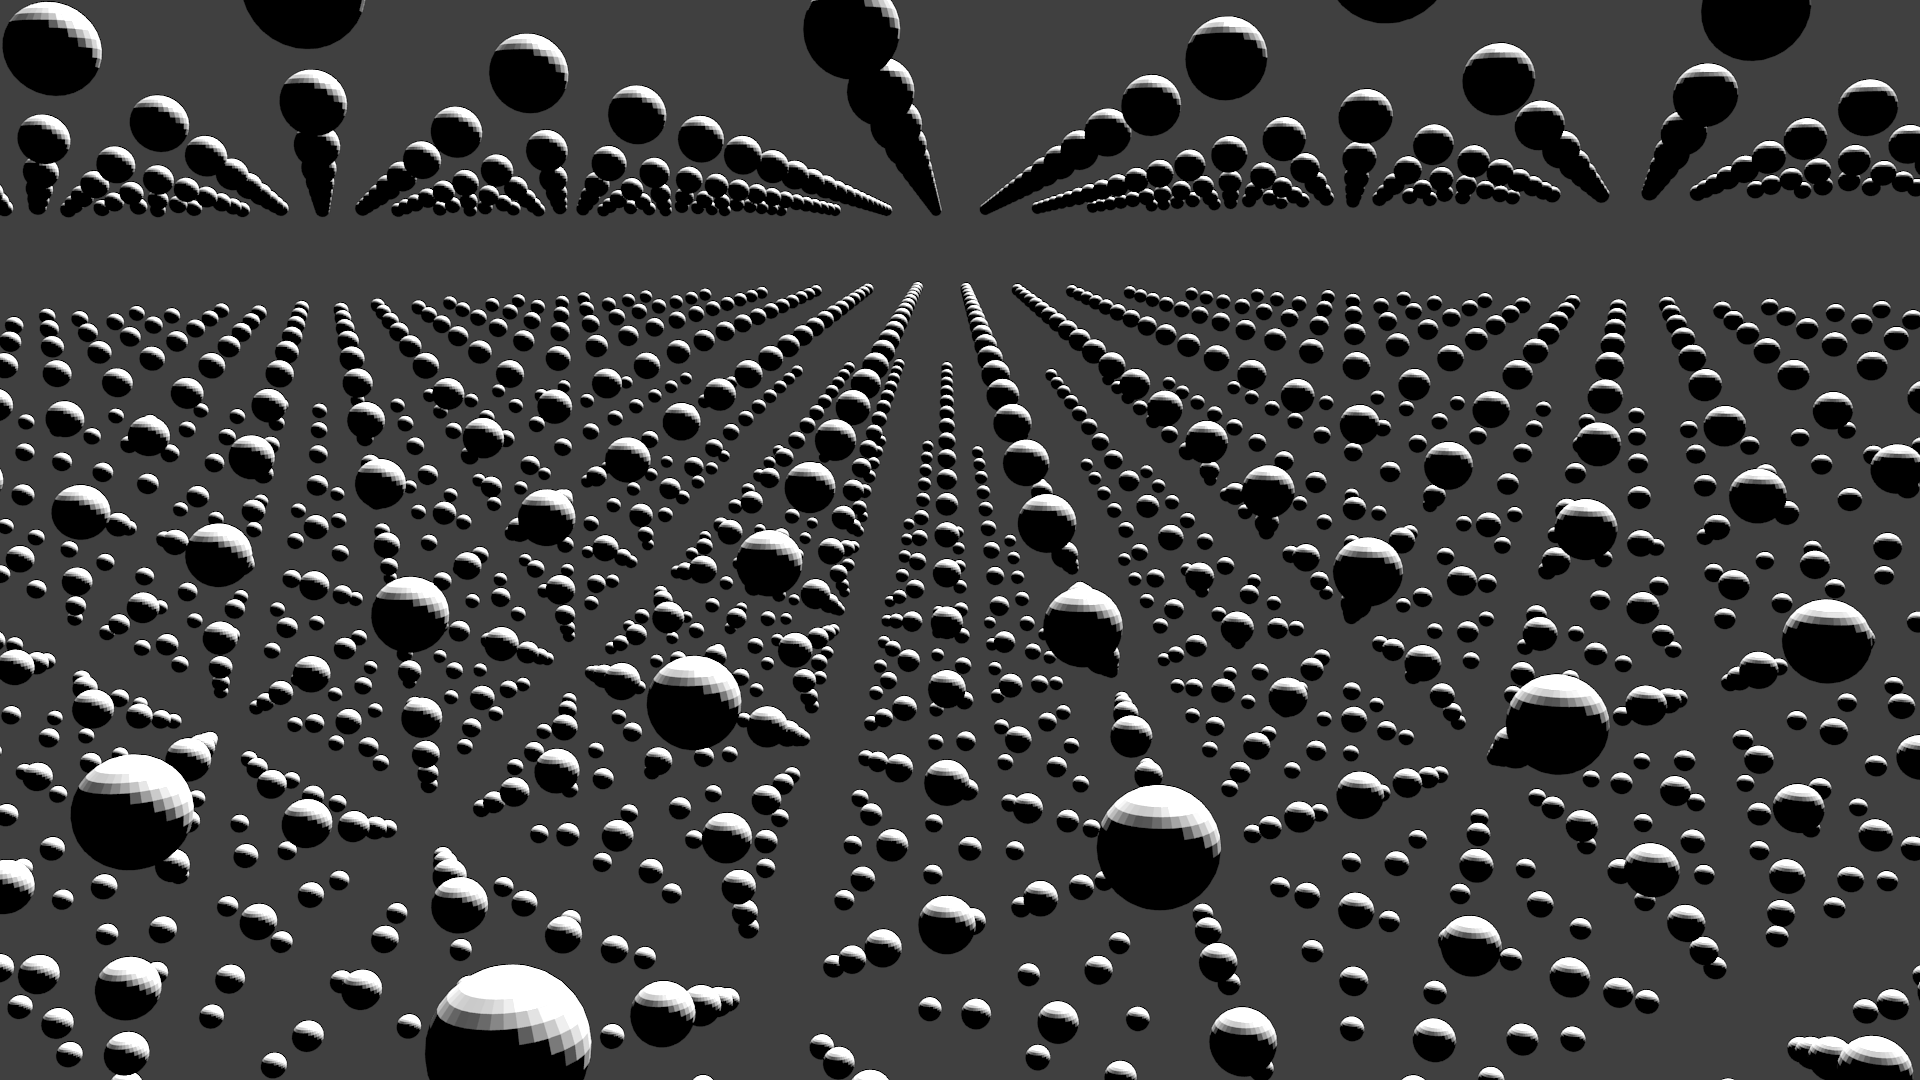
\includegraphics[width=\textwidth]{lattice.png}
\caption{A lattice in three-dimensional space}
\label{lattice_graphic}
\end{figure}

Interestingly, lattices are not only useful for cryptography, but they have numerous applications in number theory, and Minkowski proved some results on the structure of lattices already around 1900. We slightly touch one of these applications, the Minkowski-Space, later when we talk about Ring Learning with Errors.

\definition[Lattice]
A subset $L \subseteq \R^n$ with $n \in \mathbb{N}$ is called a lattice, if there exist linearly independent vectors $v_1, ..., v_t \in \R^n$ so that $L = v_1 \Z + ... + v_t \Z$. If $t = n$, the lattice is called full-rank. $n$ is called the dimension of the lattice.
\paragraph{Notation} Have $B := (v_1 | ... | v_t) \in \R^{n \times t}$. Then define the lattice $\mathcal{L}(B) := \{ Bx | x \in \Z^t \}$.

\definition[Fundamental Parallelepiped]
For a lattice $L = \mathcal{L}(B)$ with basis $B \in \R^{n \times n}$, have the fundamental parallelepiped $\mathcal{P}(B) := B [0, 1)^n \subseteq \R^n$. The fundamental parallelepiped is a 	representative system for the quotient module $\R^n / \mathcal{L}(B)$, so each point $x \in \R^n$ has exactly one representation $x = x_0 + v$ with $x_0 \in \mathcal{B}$ and $v \in L$.
\paragraph{Notation} Denote $x \mod \mathcal{P}(B) := x_0$.

\example[Easy Lattice Problems]
For cryptographic purposes, we are interested in computational problems that work on lattices. For example, given a basis $B \in \R^{n \times n}$, the following problems can be solved in polynomial time:
\begin{itemize}
\item Given $x \in \R^n$, check if $x \in \mathcal{L}(B)$
\item Given another basis $B' \in \R^{n \times n}$, check if $\mathcal{L}(B) = \mathcal{L}(B')$
\end{itemize}
These ``algebraic'' problems in lattices are usually easy (they can be solved using Gaussian Elimination). We get the hard problems needed for cryptography when we look at ``geometric'' problems, i.e.\ problems that rely on a norm in addition to the additive structure of the lattice.

\remark[Norm]
\label{lattice_norm}
Denote with $\|x\|$ the $l_2$-norm of the vector $x \in \R^n$ and denote with $\|x\|_\infty$ the $l_\infty$-norm of $x$. We also write $\langle \cdot, \cdot \rangle$ for the standard inner product on $\R^n$ resp. $\mathbb{C}^n$. 

We will also require use a ``norm'' on the $\Z$-module $(\R / q\Z)^n$, which should be the classical $l_2$ resp. $l_\infty$ norm based on the ``absolute value'' of $x \in \T_q := \R / q\Z$ defined as $| x | := \min \{ |r| | r \in \R , x = r \mod q\Z \}$, i.e.\ the absolute value of the representative of $x$ in $[ -q/2, q/2 )$. This is not a norm in the classical sense (e.g. in general $\| a x \| \neq | a | \| x \|$), but nevertheless, it will be useful.

\definition[Dual Lattice]
For a $n$-dimensional full-rank lattice $L$, define the dual lattice as $L^* := \{ x \in \R^n | \langle x, L \rangle \subseteq \Z \}$ (where $\langle x, L \rangle$ denotes $\{\langle x, y \rangle|y \in L\}$).

\remark
The dual lattice is a lattice. Obviously, it is a $\Z$-module, so we have to show that it is free. Let $L = \mathcal{L}(B)$ with a basis $B = (b_1|...|b_n) \in \text{GL}_n(\R)$. Then $(B^T)^{-1} = (b_1^*|...|b_n^*) \in \text{GL}_n(\R)$ is a basis of the dual lattice.
\subparagraph{Independent} $b_1^*, ..., b_n^*$ are linearly independent, since $B^*$ is invertible
\subparagraph{$\subseteq$} Have $x \in L^*$. Then $\langle x, b_i \rangle \in \Z$ and so $u^T := x^T B \in \Z^n$. We get
\begin{equation}
x^T = u^T B^{-1} \text{ and so } x = \left(B^{-1}\right)^T u = \left(B^T\right)^{-1} u \in  \left(B^T\right)^{-1} \Z^n = \mathcal{L}\left(B^*\right) \nonumber
\end{equation}
\subparagraph{$\supseteq$} Follows from $\langle b_i^*, b_j \rangle = \delta_{ij} \in \Z$. This holds, since 
\begin{equation}
\langle b_i^*, b_j \rangle = \left(b_i^*\right)^T b_j = \left(\left(B^T\right)^{-1}e_i\right)^TBe_j = e_i^T B^{-1}Be_j = e_i^Te_j = \delta_{ij}  \nonumber
\end{equation}

\definition[Lattice quantities]
Let $L$ be a lattice. Define 
\begin{equation}
\lambda_k(L) := \min \{ \max \{ \|x_1\|, ..., \|x_k\| \} \ | \ x_1, ..., x_k \in L \text{ linearly independent} \} \nonumber
\end{equation}
as the shortest length so that there are $k$ linearly independent vectors of at most this length in $L$. The length of a shortest, non-zero vector $\lambda_1(L)$ is also denoted by $\lambda(L)$. For a point $x \in \R^n$ define also $\kappa(x) = \kappa_L(x) \in L$ as the nearest lattice point to $x$. If $x$ is within distance $< \frac {\lambda(L)} 2$ to $L$, this is unique. We will only consider this case, but for a complete definition we might define $\kappa(x)$ as the lexicographically first lattice point among all closest ones.

\lemma
\label{lambda_dual_lattice}
For any lattice $L$, we have
\begin{equation}
\lambda_1(L^*)\lambda_n(L) \geq 1 \nonumber
\end{equation}

\begin{proof}
Let $x \in L^*$ be a vector of norm $\| x \| = \lambda_1(L^*)$ and have a basis $b_1, ..., b_n \in L$ with $\| b_i \| \leq \lambda_n(L)$. Then there is one $i$ with $\langle x, b_i \rangle \neq 0$ (otherwise all $b_i$ would be in the $n-1$ dimensional hyperplane perpendicular to $x$, a contradiction to them being a basis). We have $| \langle x, b_i \rangle | \geq 1$ since $b_i \in L, x \in L^*$ so $\langle x, b_i \rangle \in \Z$. By Cauchy-Schwarz, we get
\begin{align*}
\lambda_1(L^*)\lambda_n(L) \geq |\langle x, b_i \rangle| \geq 1 & \qedhere
\end{align*}
\end{proof}

\definition[Gaussian distribution]
For any $s > 0$, define the function
\begin{equation}
\rho_s: \R^n \to \R, x \mapsto \exp\left(-\pi\frac {\| x \|^2} {s^2}\right) \nonumber
\end{equation}
We extend $\rho$ to sets $K \subseteq L$ for a lattice $L \subseteq \R^n$ by $\rho_s(K) := \sum_{x \in K} \rho_s(x)$. The sum is finite since $\int_{\R^n} \rho_s(x) dx = s^n$ is finite.

We also have that $\frac 1 {s^n} \rho_s$ is a probability density function, and the corresponding distribution is the (continuous) normal distribution $\nu_s$ with standard deviation $s/\sqrt{2\pi}$. More interesting however is the discrete gaussian distribution $D_{L, s}$ on a lattice $L$ and width $s$, which we define by the probability mass function
\begin{equation}
f(x) = \frac {\rho_s(x)} {\rho_s(L)} \nonumber
\end{equation}

\definition[Smoothing Parameter]
 For a lattice $L$ and some $\epsilon > 0$, let the smoothing parameter $\eta_\epsilon(L)$ be the smallest $s > 0$ so that $\rho_{1/s}(L^* \setminus \{ 0 \}) \leq \epsilon$.
\\\\
The following propositions show why this is called ``smoothing parameter''. Intuitively, the smoothing parameter represents the amount of noise that is required to ``smooth'' out the discrete structure of the lattice.

\lemma
\label{smoothing_parameter_smooth_discrete_structure}
For a lattice $L = \mathcal{L}(B),\ \epsilon > 0$ and $r \geq q \eta_\epsilon(L) = \eta_\epsilon(q L)$ we get for a random variable $v \sim D_{L, r}$ that $v \mod qL$ is within statistical distance $2\epsilon$ from a uniform distribution on $B\Z_q^n \cong L/qL$.

In particular, $B^{-1}v$ is almost uniform in $\Z_q^n$.

\begin{proof} \noqed
This lemma follows from \cite[3.8]{Reg}.
\end{proof}

\lemma
\label{smoothing_parameter_smooth_discrete_gaussian}
For a lattice $L,\ u \in \R^n$ and $r, s > 0$, define the random variables $v \sim D_{L + u, r}$ and $e \sim \nu_s$. If
\begin{equation}
rs / \sqrt{r^2 + s^2} \geq \eta_\epsilon(L) \nonumber
\end{equation}
for some $\epsilon < \frac 1 2$, the statistical distance between $v + e$ and $\nu_{\sqrt{r^2 + s^2}}$ is at most $4\epsilon$.

\begin{proof} \noqed
See \cite[3.9]{Reg}.
\end{proof}

\lemma
\label{smoothing_parameter_lower_bound}
For a lattice $L,\ c > 0$ and $\epsilon(n) \in o(1)$ have for sufficiently large $n$ that
\begin{equation}
\eta_{e(n)}(L) > \frac c {\lambda_1(L^*)} \geq \frac {c\lambda_n(L)} n \nonumber
\end{equation}

\begin{proof} \noqed
See \cite[2.13]{Reg}.
\end{proof}

\lemma
\label{smoothing_parameter_upper_bound}
For a lattice $L$ we have with $\epsilon = 2^{-n}$ that
\begin{equation}
\eta_{e}(L) \leq \frac {\sqrt{n}} {\lambda_1(L^*)} \nonumber
\end{equation}

\begin{proof} \noqed
See e.g. \cite[2.11]{Reg}.
\end{proof}

\lemma
\label{gaussian_length_bound}
For a lattice $L$ and $r > 0$ we have
\begin{equation}
\rho_r(L \setminus \sqrt{n}rB_n) < 2^{-2n} \rho_r(L) \nonumber
\end{equation}
where $\sqrt{n}rB_n = \{x \in L | \|x\| < r\sqrt{n}\}$ is the set of lattice points with norm smaller than $r\sqrt{n}$. In other words, a point from $D_{L, r}$ has norm greater $r\sqrt{n}$ with only negligible probability.

\begin{proof} \noqed
See \cite[1.5(i)]{Ban}.
\end{proof}

\definition[Computational Lattice Problems]
\label{lattice_problems}
Let $\gamma(n) \geq 1$. Define the following computational problems:
\begin{itemize}
\item (Shortest Vector Problem, $\mathrm{SVP}_\gamma$) Given a basis of a full-rank lattice $B \in \R^{n \times n}$, find a short lattice vector, i.e.\ find $x \in \mathcal{L}(B)$ so that $\|x\| \leq \gamma \lambda_1(\mathcal{L}(B))$.
\item (Shortest Independent Vector Problem, $\mathrm{SIVP}_\gamma$) Given a basis of a full-rank lattice $B \in \R^{n \times n}$, find independent lattice vectors $v_1, ..., v_n \in \mathcal{L}(B)$ that are quite short, i.e.\ $\|v_i\| \leq \gamma \lambda_n{\mathcal{L}(B)})$.
\item (Closest Vector Problem, $\mathrm{CVP}_\gamma$) Given a basis of a full-rank lattice $B \in \R^{n \times n}$ and $a \in \R^n$, find a lattice point that is close to $x$, i.e.\ find $x \in \mathcal{L}(B)$ with $\|x - a\| \leq \gamma \|\kappa(x) - a\|$ where $y \in \mathcal{L}(B)$ is the closest lattice point to $x$.
\item ($\mathrm{GapSVP}_\gamma$) Given a basis of a full-rank lattice $B \in \R^{n \times n}$ so that either $\lambda(\mathcal{L}(B)) < 1$ or $\lambda(\mathcal{L}(B)) \geq \gamma$, find out what is the case.
\item (Bounded Distance Decoding, $\mathrm{BDD}_\gamma$) Given a basis of a full-rank lattice $B \in \R^{n \times n}$ and $a \in \R^n$ with $\|\kappa(a) - a\| < \gamma$, find $\kappa(a)$.
\end{itemize}
We also write $\mathrm{BDD}_{L, \gamma}$ for the bounded distance decoding problem in a fixed lattice $L$.

\remark[Difficulty]
The difficulty of those problems depends on the choice of the parameter $\gamma$. Using the LLL algorithm for example, one can efficiently compute for a given lattice $L = \mathcal{L}(B)$ a basis with relatively small vectors $b'_1, ..., b'_n$. In particular one can get 
\[\|b'_1\| \leq \gamma\lambda(L) \text{ for } \gamma = 2^{\frac 1 2 (n-1)}\]
and so solve SVP$_\gamma$ for exponential $\gamma$. 
On the other hand, SVP$_\gamma$, CVP$_\gamma$, GapSVP$_\gamma$ and BDD$_\gamma$ are conjectured to be hard for polynomial or smaller $\gamma$ (resp. bigger $\gamma$ in case of BDD), and there are various results for smaller $\gamma$. For example, GapSVP$_\gamma$ for $\gamma \in O(n^{c/\log\log n})$ is NP-hard under randomized reductions.

\example
\begin{equation}
\mathrm{SVP}_\gamma \leq_p \mathrm{CVP}_\gamma
\end{equation}

\begin{proof}
Let $B \in \R^{n \times n}$ be a basis and $L := \mathcal{L}(B)$. Let $x \in L \setminus \{0\}$ be the shortest vector in $L$. 
$\Rightarrow{} x = Ba$ for $a \in \Z^n$. 

We have $a_j \equiv 1 \ (\text{mod} \ 2)$ for some $j$, since otherwise $\frac 1 2 a \in \Z^n$ and so $\frac 1 2 B a \in L$ would be shorter than $x$. So the following algorithm finds $x$:
\begin{itemize}
\item For $i$ in $\{1, ..., n\}$
\begin{itemize}
\item Calculate basis of $L_i := \{ Ba + Be_i | a \in \Z^n, a_i \equiv 1 \ (\text{mod} \ 2) \}$
\item Use oracle to find approximation to closest lattice point $x_i$ to $Be_i$
\end{itemize}
\item Output the shortest of all $x_i - Be_i$
\end{itemize}
Since $a_j \equiv 1 \ (\text{mod} \ 2)$, we have $x + Be_j \in L_j$. As $x$ is the closest nonzero vector to $0$ in $L$, $x + Be_j$ is the closest vector $\neq Be_j$ to $Be_j$ in $L$. So the oracle will yield $x + Be_j \in L_j \subseteq L$, because $Be_j \not \in L_j$. Therefore, $x_j - Be_j = x$ and the algorithm outputs $x$ or another vector of the same length. \qedhere
\end{proof}

% LEARNING WITH ERRORS

\chapter{Learning with Errors}

Let $q \in \Z, q \geq 2$ be a prime number and have $\Z_q := \Z / q\Z$.

\motivation
While the lattice problems we looked at in the previous section are considered hard, they are not very well suited for cryptographic applications. One reason is that all the considered vectors are continuous and have (in principle) unbounded length. However, it is sufficient to only work with points on a discrete grid in the fundamental parallelepiped, which is easier and more efficient to implement. This leads to the Learning with Errors problem, which can be characterized as solving a noisy system of linear equations in $\Z_q$, i.e.\ find $x$ given
\begin{equation}
\begin{split}
b_1 &\approx a_{11} x_1 + ... + a_{1n} x_n \\
& \vdots \\
b_n &\approx a_{m1} x_1 + ... + a_{mn} x_n \nonumber
\end{split}
\end{equation}
Even though it is not immediately visible, this problem has a strong connections to lattices, especially with the bounded distance decoding problem. The advantage of LWE is that it can be implemented very efficiently, and it has a natural decision version that is as hard as LWE and very well suited for building public-key cryptosystems. Additionally, solving average case LWE is already sufficient to solve any instance of the problem, which is a singular property of lattice based cryptosystems. These results are not hard to prove, and we will do so in this section. The connection to the discussed lattice problems is more so, and we will consider it in the next section.

\definition
Define the $\Z$-module $\T_q := \R / q\Z$ with the submodule $\Z_q$ with the ``norm''-like operation defined in \ref{lattice_norm}. Let $\Psi_\alpha := \nu_{\alpha q} \mod q$ be the centered normal distribution with standard deviation $\alpha q / \sqrt{2\pi}$ modulo $q$ on $\T_q$.

\definition[Learning with Errors]
We define two variants of LWE:
\paragraph{Continuous}
For a probability distribution $\chi$ on $\T_q$ and some $s \in \Z_q^n$, define the LWE distribution $A_{s, \chi}$ on $\Z_q^n \times \T_q$ as the probability distribution that results from choosing an $a \in \Z_q^n$ uniformly, $e \sim \chi$ and outputting $(a, \langle a, s \rangle + e)$. We will often use $\chi = \Psi_\alpha$.

\paragraph{Discrete}
For a probability distribution $\chi$ on $\Z_q$ and some $s \in \Z_q^n$, define the LWE distribution $A_{s, \chi}$ on $\Z_q^n \times \Z_q$ as the probability distribution that results from choosing an $a \in \Z_q^n$ uniformly, $e \sim \chi$ and outputting $(a, \langle a, s \rangle + e)$. We will often use $\chi = \bar{\Psi}_\alpha$, where $\bar{\Psi}_\alpha := \lfloor \Psi_\alpha \rceil$ is $\Psi_\alpha$ rounded to the nearest integer.
\\\\
Then the (average case) LWE problem $\mathrm{LWE}_{q, \chi}$ is defined as: Given access to samples from $A_{s, \chi}$ for a uniformly chosen $s \in \Z_q^n$, retrieve $s$. We also write $\mathrm{LWE}_{q, \alpha}$ for $\mathrm{LWE}_{q, \Psi_\alpha}$.

If the number of samples is a fixed $m \in \mathbb{N}$, then LWE is often written as: Given $(A, b = As + e)$, find $s$ where $A \in \Z_q^{m \times n}$ is a uniformly chosen matrix and $e \sim \chi^m$ is a random vector.

\remark
We define both versions of LWE, as the discrete one is better suited for computations, while it is often mathematically cleaner to work with a continuous error distribution. However, when we get samples $(A, b) \sim A_{s, \Psi_\alpha}$, then $(A, \lfloor b \rceil)$ is distributed like $A_{s, \bar{\Psi}_\alpha}$, so the discrete variant of LWE (which can be implemented) is at least as secure as the continuous one. One can also prove the opposite way, with only a slight increase in the amount of error.

\remark[Checking LWE solutions]
By definition, a given $s \in \Z_q^n$ is a valid LWE solution for samples $(A, b)$ if $e := b - As$ is distributed according to $\chi^m$. While this condition follows directly from the definition, it is not so easy to work with. Instead, we sometimes consider a solution $s \in \Z_q^n$ a valid LWE solution, if $\| e \|_\infty = \| b - As \|_\infty \leq \alpha q\sqrt{n}$. This holds for all samples from $\Psi_\alpha^m$ with high probability: 

Let $e_1, ..., e_m \sim \Psi_\alpha$ be iid. random variables. Then $\| e \|$ is distributed according to the $\chi$-distribution, and using properties of the $\chi$-distribution, we get that $\Pr[\| e \| \geq \alpha q\sqrt{n}]$ is negligible. Since $\| e \|_\infty \leq \| e \|$, we get that $\| e \|_\infty \leq \alpha q\sqrt{n}$ with high probability.

In particular, this version of LWE is not less secure than the classic one.

\proposition{LWE solution is unique}
\label{unique_lwe_solution}
Given LWE samples $(A, b:=As+e)$, where $A \in \Z_q^{m \times n}$ uniform and $e$ chosen accordingly to $\bar{\Psi}_\alpha^m$, we have $\Pr[\exists s' \in \Z_q^n \setminus \{s\}: \|As'-b\|_\infty \leq \beta q] \leq q^n(2\beta + 1/q)^m$.

In particular, with high probability there is at most one LWE solution $s$ if $m \in \omega(n\log q)$, $q \in \omega(1)$ and $\beta \leq \frac 1 2 - \epsilon$ for $\epsilon > 0$.

\begin{proof}
Consider a fixed $s$, let $e \sim \chi^m$ be a random variable and let
\begin{equation}
A = \begin{pmatrix}
	... a_1 ... \\
	\vdots \\
	... a_m ...
	\end{pmatrix}
\nonumber
\end{equation}
be a random variable describing the choice of $A$ in the LWE samples. We get:
\begin{equation}
\begin{split}
&\Pr[\exists s' \in \Z_q^n \setminus \{s\}: \| As' - b \|_\infty \leq \beta q] \\
= & \Pr[\exists s' \in \Z_q^n \setminus \{s\}: \| As' - As - e \|_\infty \leq \beta q] \\
\leq & \sum_{s' \in \Z_q^n \setminus \{s\}}\Pr[\|As' - As - e\|_\infty \leq \beta q] \\
= & \sum_{s' \in \Z_q^n \setminus \{s\}}\Pr[\forall i \in \{1, ..., m\}: |(A(s' - s) - e)_i| \leq \beta q] \\
= & \sum_{s' \in \Z_q^n \setminus \{s\}}\Pr[\forall i \in \{1, ..., m\}: |\langle a_i, s'-s \rangle - e_i| \leq \beta q]
\end{split} \nonumber
\end{equation}
Since the $a_i$ are independent uniformly distributed, the $\langle a_i, s'-s \rangle - e_i$ are also independent and uniformly distributed (since $s' - s \neq 0$ is a constant). It follows:
\begin{equation}
\begin{split}
&\Pr[\exists s' \in \Z_q^n \setminus \{s\}: \| As' - b \|_\infty \leq \beta q] \\
\leq & \sum_{s' \in \Z_q^n \setminus \{s\}} \prod_{i = 0}^m \Pr[|\langle a_i, s'-s \rangle - e_i| \leq \beta q] \\
= & \sum_{s' \in \Z_q^n \setminus \{s\}} (2 \beta + 1/q)^m \\
\leq & q^n(2\beta + 1/q)^m
\end{split} \nonumber
\end{equation}
This holds for every fixed $s$, so it holds also for some uniformly distributed random $s$.

If $m \in \omega(n\log q), 2\beta \leq 1 - \epsilon$, get that $2\beta + 1/q \leq 1 - \epsilon$ for sufficiently large $n$, and so
\begin{align*}
q^n(2\beta + 1/q)^m \leq e^{n\log q}(2\beta + 1/q)^{\omega(n\log q)} = e^{n\log q - \omega(n\log q)} \text{ negligible.} & \qedhere
\end{align*}
\end{proof}

\proposition{Worst case to average case reduction}
\label{average_to_worst}
A singular property of some lattice based problems is that they allow randomized self reductions, so an instance of the problem can be reduced to solving another, random instance of the problem. For LWE this means:

Assume we have access to an oracle that solves average case $\mathrm{LWE}_{q, \chi}$, i.e.\ given samples of $A_{s, \chi}$ for a uniformly chosen $s \in \Z_q^n$, can retrieve $s$ with probability exponentially close to $1$ (over the randomness of $s$ and the samples). Then we can solve worst case $\mathrm{LWE}_{q, \chi}$, i.e.\ given samples of $A_{s, \chi}$ for any $s \in \Z_q^n$, can retrieve $s$ with probability exponentially close to $1$ (over the randomness of the samples).

In particular, this reduction is lattice-preserving, so on input samples $(A, b)$, it calls the oracle with $(A, b')$. Therefore, the reduction remains valid when choosing $A$ from another distribution (in both problems).

\begin{proof}
Consider the algorithm that, on input $(A, b)$ does the following:
\begin{itemize}
\item Choose uniformly random $d \sim \Z_q^n$
\item Call oracle on $(A, b + Ad)$ to get $s'$ and output $s = s' - d$, where $(A, b)$ are the input samples
\end{itemize}
The samples $(A, b + Ad)$ generated in the second step are distributed according to $A_{s',  \chi}$ with secret $s' = s + d$, as $Ad + b = Ad + As + e = A(s + d) + e$. We chose $d$ uniformly and independently of $s$, so $s' = s + d$ is uniformly distributed, and the oracle will correctly give us $s'$ when called on $(A, b + Ad)$. As a result, we have found $s = s' - d$.\qedhere
\end{proof}

\definition[Decision LWE]
Consider the decision version of LWE for a probability distribution $\chi$: Given access to samples from $A_{s, \chi}$ for a fixed uniformly chosen $s \in \Z_q^n$ or samples from $(a, u)$ where $a \in \Z_q^n$ and $u \in \Z_q$ resp. $u \in \T_q$ are uniformly chosen, determine what is the case.

\proposition{Search to decision reduction}
\label{decision_to_search}
Let $q \in O(\mathrm{poly}(n))$. Then the decision LWE problem is not easier than the search version, i.e.\ for a probability distribution $\chi$ on $\T_q$, given an oracle that can distinguish samples from $A_{s, \chi}$ for a uniformly chosen $s \in \Z_q^n$ and samples $(a, u)$ with uniform $a \in \Z_q^n$ and $u \in \T_q$ (with a polynomial distinguishing probability gap $\Delta$), we can find solve $\mathrm{LWE}_{q, \chi}$.

This reduction is secret-preserving, so on input samples $(A, As + e)$ it calls the oracle on samples $(A', A's + e)$. Therefore, this reduction remains valid when choosing $s$ from another distribution than the uniform one (in both problems).

\begin{proof}
Let $m \in O(\mathrm{poly}(n))$ be the maximum count of samples the oracle needs. Consider the algorithm $F$ that does the following:
\begin{itemize}
\item For $k \in \{ 1, ..., n\}$ and each $r \in \Z_q$ do:
\begin{itemize}
\item Check if $s_k = r$ by repeating this procedure sufficiently often:
\begin{itemize}
\item Select $d \in \Z_q^m$ uniformly random
\item Get $m$ input samples $(A, b)$ with $A \in \Z_q^{m \times n}$
\item Construct the matrix $A'$ with $d$ in the k-th column
\[ A' := \begin{pmatrix}
	0 & & d_1 & & 0 \\
	\vdots & ... & \vdots & ... & \vdots \\
	0 & & d_m & & 0 \\
         \end{pmatrix} \]
\item Call the oracle with samples $(A + A', b + dr)$. If we got ``not uniform'', then $s_k = r$, otherwise $s_k \neq r$
\end{itemize}
\item Set $s_k = r$ if the check returned true
\end{itemize}
\end{itemize}
\subparagraph{Show} The check procedure will distinguish situations with $s_k = r$ and $s_k \neq r$ with acceptance probability gap at least $\Delta$ over the choices of $d$, the samples $(A, b)$ and the coins of the oracle.

Let $p$ be the probability that the oracle will output ``not uniform'' on a uniform sample. For a given $k \in \{ 1, ..., n\}$, we have $(A + A')s = As + ds_k$.

\subparagraph{If} $r = s_k$, then $(A + A', b + dr)$ is distributed according to $A_{s, \chi}$, since $A + A'$ is uniform and $(A + A')s = As + dr$.
\\$\xRightarrow{}$ The oracle will return ``not uniform'' with probability $p + \Delta$ and the algorithm will find $s_k = r$ with probability $p + \Delta$.

\subparagraph{If} $r \neq s_k$, then $b + dr = As + e + dr = (A + A')s + e + d(r - s_k)$. Since $r - s_k \neq 0$ and $d$ uniform, $d(r - s_k)$ and therefore both $b + dr = (A + A')s + e + d(r - s_k)$ and $A + A'$ are uniform.
\\$\xRightarrow{}$ The oracle will return ``uniform'' with probability $1 - p$ and the algorithm will find $s_k \neq r$.

By repeating the check procedure (with different $d$) and checking if significantly more resp. less than $p + \frac 1 2 \Delta$ cycles accepted, the algorithm can determine whether $s_k = r$ with very high probability for each $r$ and therefore find $s_k$ and $s$.\qedhere
\end{proof}

\proposition{Secret from Error Distribution}
\label{secret_error_distribution}
LWE becomes no easier when we draw $s$ from the error distribution $\chi$ on $\Z_q$ instead of the uniform distribution on $\Z_q^n$. In other words: Given an oracle that, given samples from $A_{s, \chi}$, where $s \sim \chi$ is random, can find $s$, we can solve $\mathrm{LWE}_{q, \chi}$ efficiently.

\begin{proof}
The idea in this proof is that we can request more samples and ``eliminate'' the secret from the formula. Then a part of the error takes the place of the secret, and we can find it using the oracle. When we know the error, we can find the secret using gaussian elimination.

Assume the oracle requests $m$ samples. Then consider the algorithm that, on $m + n$ input samples $(A_1, b_1), (A_2, b_2)$ for $A_1 \in \Z_q^{m \times n}, A_2 \in \Z_q^{n \times n}$ calls the oracle on 
\begin{equation}
(A_1 A_2^{-1}, A_1 A_2^{-1} b_2 - b_1) \nonumber
\end{equation} and returns $A_2^{-1} (b_2 - s')$ where $s'$ is the output of the oracle. We can do so, as $A_2$ is invertible with probability of $1 - 1/q$: Since $\#\det^{-1}(\{k\}) = \#\det^{-1}(\{l\})$ for $k, l \in \Z_q$, we have that $\det(A_2)$ is uniform on $\Z_q$, and therefore the probability that $\det(A_2) = 0$ is $1/q$.

For the input, we have $A_1 s + e_1 = b_1$ and $A_2 s + e_2 = b_2$. We claim that the generated samples are distributed according to $A_{e_2, \chi}$ where $e_2 \sim \chi$, so the oracle will yield $s' = e_2$ and we will output $A_2^{-1} (b_2 - e') = A_2^{-1} A_2 s = s$. We have
\begin{equation}
A_1 A_2^{-1} b_2 - b_1 = A_1 A_2^{-1} (A_2 s + e_2) - A_1 s - e_1 = A_1 A_2^{-1} e_2 - e_1 \nonumber
\end{equation}
Since $A_1$ is uniform and independent of $A_2$ and $A_2$ is invertible, $A_1 A_2^{-1}$ is uniform on $\Z_q^{m \times n}$. Obviously $e_1$ and $s' = e_2$ are drawn from $\chi^m$ resp. $\chi^n$, so we have generated valid samples of $A_{e_2, \chi}$. \qedhere
\end{proof}

% HARDNESS LWE

\chapter{Hardness of LWE}

\motivation
While LWE has some properties that make it well suited for cryptographic applications, it is not as established as many well-known cryptographic problems, and there is much less evidence for its hardness. Therefore, it would be desirable to base its security on some problem that has been examined in more detail and whose hardness is better understood. In this section, we will present such a reduction to one of the standard lattice problems that we have already seen, namely the approximation of the short vector problem. This also demonstrates the connection to lattices. An interesting point is that this reduction is quantum, so we assume the quantum hardness of the short vector problem. There are also classical reductions, but they impose restrictions on the parameters and are less central to our understanding of LWE (e.g. \cite{ClassicalReduction}). We will also present a cryptosystem that already has some similarities with Crystals-Kyber.

\definition
For $\alpha > 0$, consider also the following variant $\mathrm{LWE}_{q, \leq \alpha}$ of worst case LWE: For any $s \in \Z_q^n$ and any (unknown) $\beta \leq \alpha$, given samples from $A_{s, \Psi_\beta}$, retrieve $s$.

\proposition{Unknown to constant error variance reduction}
\label{lwe_leq_alpha_lwe_alpha}
Given an oracle for worst case LWE with error distribution $\Psi_\alpha$, we can solve $\mathrm{LWE}_{q, \leq \alpha}$.

\begin{proof}
The idea of this proof is the following lemma from \cite[2.2]{Reg}:
\paragraph{Lemma} For any $\alpha > 0$ and $0 < \epsilon \leq \alpha$, we have that the statistical distance between $\Psi_\alpha$ and $\Psi_{\alpha + \epsilon}$ is at most $9\epsilon / \alpha$.
\\\\
Let $p(n) \in (0, 1]$ be the success probability of the oracle and $m \in O(\mathrm{poly}(n))$ the amount of samples the oracle needs. Then define 
\begin{equation}
\epsilon := \frac 1 {18m} p \alpha \quad \text{ and } \quad N = \alpha/\epsilon \in O(\mathrm{poly}(n)) \nonumber
\end{equation}
Given samples $(A, b) \sim A_{s, \beta}$ we can now find $s$ by calling the oracle on $(A, b + e_k)$ for each $k \in \{ 0, ..., N \}$, where $e_k \sim \nu_{k\epsilon}^m$ is a normal random variable. If one of these calls returns the correct secret (we can check that), this is our result. We have to show that with high probability, this happens. 

Let $k$ be the smallest number with $k\epsilon \geq \alpha - \beta$. We claim that with high probability, the oracle returns the correct secret when called on $(A, b + e_k)$. The random variable $(A, b + e_k)$ is distributed like $A_{s, \Psi_{\beta + k\epsilon}}$, and by the lemma, the statistical distance to $A_{s, \Psi_\alpha}$ is at most $9\epsilon / \alpha$. Therefore, the statistical distance between $A_{s, \Psi_{\beta + k\epsilon}}^m$ and $A_{s, \Psi_\alpha}^m$ is at most $m 9\epsilon / \alpha = \frac 1 2 p$. Since applying the oracle cannot increase the statistical distance, the output of the oracle on $(A, b + e_k)$ is within distance $\frac 1 2 p$ of the output on valid samples $(A', b') \sim A_{s, \Psi_\alpha}^m$, and therefore, we find the secret with probability at least $\frac 1 2 p$. \qedhere
\end{proof}

\theorem{SIVP to LWE reduction}
\label{hardness_lwe}
For $\alpha q \geq 2\sqrt{n}$, there is a quantum reduction from worst case $\mathrm{LWE}_{q, \leq \alpha}$ to worst case $\mathrm{SIVP}_{2n\sqrt{2n}/\alpha}$. Using some stronger bounds on $\eta_\epsilon(L)$, \cite{Reg} even proves the reduction to  $\mathrm{SIVP}_{2n\sqrt{2\omega(\log(n))}/\alpha}$.

\subsection{Remark}
We will present a summary of the proof given in \cite{Reg}. This proof relies heavily on some technical results about the smoothing parameter and the discrete gaussian distribution that go beyond the scope of this work. Therefore, we will only sketch some edge parts of the argument, but we try to present the main ideas formally correct (namely the use of the LWE oracle and the quantum part of the reduction).

\begin{proof}
The heart of the proof is the following lemma:

\lemma[Improvement of gaussian samples using LWE]
\label{recursive_step}
Let $\epsilon$ be negligible, $\alpha \in (0, 1)$ and $r > \sqrt{2}q\eta_\epsilon(L)$. Given an oracle for $\mathrm{LWE}_{q, \leq \alpha}$ and samples from $D_{L, r}$ (as many as the oracle needs), we can efficiently generate samples from $D_{L, r\sqrt{n}/\alpha q}$. The generated samples are stochastically independent of the input samples and of each other.

\begin{proof}
We begin with stating the following lemma on the inner product with discrete gaussian vectors:
\paragraph{Lemma 1}
For a lattice $L,\ z, u \in \R^n,\ r, \alpha > 0$ and $\epsilon \leq \frac 1 2$ with 
\begin{equation}
1 / \sqrt{\frac 1 {r^2} + \frac {\| z \|^2} {\alpha^2}} \geq \eta_{\epsilon}(L) \nonumber
\end{equation}
we have for random variables $v \sim D_{L + u, r}$ and $e$ normally distributed with standard deviation $\alpha/\sqrt{2\pi}$ that the $\langle z, v \rangle + e$ is within statistical distance $4\epsilon$ to
\begin{equation}
\nu_{\sqrt{(r\| z \|)^2 + \alpha^2}} \nonumber
\end{equation}
In particular, we get that $\langle z, qv \rangle + qe \mod q$ is within statistical distance $4\epsilon$ to $\Psi_\alpha$.

\begin{proof} \noqed See e.g. \cite[3.10]{Reg}. 
    
    Intuitively, this lemma says that the scalar product of a constant vector with a vector drawn from the discrete gaussian distribution is distributed like an LWE error.
\end{proof}

Let $L = \mathcal{L}(B)$ and $L^* = \mathcal{L}(B^*)$ with $B^* = \left(B^{-1}\right)^T$. For this proof, we also require a variant of the BDD problem:
\subsection{Definition $\mathrm{BDD}_{L, \gamma}^q$}
Define the problem as: Given $x \in \R^n$ close to $L$, calculate the coefficients of $\kappa(x)$ modulo $q$, i.e.\ calculate $s \mod q$ where $Bs = \kappa(x)$ when given a point $x$ close to $L$ (within distance $\gamma$)
\\\\
Then proof consists of the following parts:
\begin{itemize}
\item Construct an oracle for $\mathrm{BDD}_{L^*, \alpha q / \sqrt{2}r}^q$.
\item Construct an oracle for $\mathrm{BDD}_{L^*, \alpha q / \sqrt{2}r}$.
\item Using this, quantumly generate samples from $D_{L, r\sqrt{n}/\alpha q}$.
\end{itemize}

\subsection{Oracle for $\mathrm{BDD}_{L^*, \alpha q / \sqrt{2}r}^q$}
Let $v_1, ..., v_n \in L$ denote the samples from $D_{L, r}$, so have $v_1, ..., v_n$ iid. random variables with $v_i \sim D_{L, r}$. On input $x \in \R^n$ with $\| x - \kappa(x) \| \leq \alpha q / r\sqrt{2}$ define
\begin{equation}
\begin{split}
s = \left(B^*\right)^{-1} \kappa(x) = B^T \kappa(x) &\in \Z^n \quad \text{ since } \quad \kappa(x) \in L^* \\
a_i = B^{-1} v_i &\in \Z^n \nonumber
\end{split}
\end{equation}
and get
\begin{equation}
\langle a_i, s \rangle = \langle B^{-1}v_i, B^T \kappa(x) \rangle = \langle v_i, \kappa(x) \rangle = \langle v_i, x \rangle + \langle v_i, \kappa(x) - x \rangle \nonumber
\end{equation}
The statistical distance between $a_i \mod q$ and a uniform random variable on $\Z_q^n$ is negligible by \ref{smoothing_parameter_smooth_discrete_structure}.
Now we condition on a fixed $a_i \mod q$. We get that $v_i / q \sim D_{L + Ba_i / q, r / q}$ and
\begin{equation}
1 / \sqrt{\frac {q^2} {r^2} + 2\frac {\| \kappa(x) - x \|^2} {\alpha^2}} \geq 1 / \sqrt{\frac {q^2} {r^2} + 2 \frac {\alpha^2 q^2} {\alpha^2 2 r^2} } = \frac r {\sqrt{2}q} > \eta_\epsilon(L) \nonumber
\end{equation}
so we can apply lemma 1 with $u = Ba_i / q$ and get that $\langle v_i / q, \kappa(x) - x \rangle + e$ is distributed according to $\nu_\beta$ where $e \sim \nu_{\alpha / \sqrt{2}}$ is a normal random variable with standard deviation $\alpha / 2\sqrt{\pi}$ and $\beta^2 = (r\| x - \kappa(x) \| / q)^2 + (\alpha/\sqrt{2})^2 \leq \alpha^2$. Since this holds conditioned on any arbitrary $a_i$, the error random variable $\langle v_i / q, \kappa(x) - x \rangle + e$ is also independent from $a_i$. Therefore, $(a_i \mod q, \langle v_i, x \rangle + qe \mod q)$ are valid samples of $A_{s, \Psi_\beta}$ and our oracle can retrieve $s \mod q$.

\subsection{Oracle for $\mathrm{BDD}_{L^*, \alpha q / \sqrt{2}r}$}
The idea is to find the digits of the coefficients in the base $q$ by repeatedly applying the oracle to new points. Let $x \in \R^n$ with $\| x - \kappa(x) \| \leq \alpha q/\sqrt{2}r$ be the input. Denote by $s$ the coefficients of $\kappa(x)$, i.e. $s = B^T \kappa(x)$. Now define
\begin{equation}
\begin{split}
x_0 &= x \\
x_{i + 1} &= \frac {x_i - B (s_i \mod q)} q \\
s_{i} &= \left\lfloor \frac s {q^i} \right\rfloor = \frac {s - (s \mod q^i)} {q^i} \in \Z^n \nonumber
\end{split}
\end{equation}
Then $\kappa(x_i) = Bs_i$ by induction, since for $x'_i = x_i - B (s_i \mod q)$ we get $x'_i - x_i = B (s_i \mod q) \in L$ so
\begin{equation}
\kappa(x'_i)  = \kappa(x_i) - B(s_i \mod q) = B\left(s_i - (s_i \mod q)\right) = B q \left\lfloor \frac s {q^{i + 1}} \right\rfloor = Bqs_{i + 1} \nonumber
\end{equation}
Since $\| a - \kappa_\Lambda(a) \| \leq \| a - \kappa_\Gamma(a) \|$ if $\Gamma$ is a sublattice of $\Lambda$, we get $\kappa_{qL}(x'_i) = Bqs_{i+1}$ and therefore
\begin{equation}
\kappa(x_{i + 1}) = \kappa_L\left(\frac {x'_i} q\right)  = \kappa(x_{i + 1}) = Bs_{i + 1} \nonumber
\end{equation}
Using this and the oracle, we can also calculate $x_{i + 1}$ and so $(s_{i + 1} \mod q)$ given $x_i$ and $s_i \mod q$. By repeating this, we get $s_i \mod q$ for any $i$. Now we find $s$ by using that $s = \sum_i s_i \mod q$.

\subsection{Generate sample of $D_{L, r\sqrt{n}/\alpha q}$}
\paragraph{Overview} Some readers might not be used to quantum computation, so an elaborate high-level overview about this part will be presented before we come to the technical details.
The main idea is that the (continous) fourier transformation transforms a distribution of repeated wide gaussians on the dual lattice to a distribution of the wanted (narrow) discrete gaussian on $L$. With ``distribution of repeated gaussians'' we mean the distribution resulting from choosing a lattice point and adding some (continous) gaussian noise, see figure \ref{repeated_gaussians}.
\begin{figure}[ht]
\centering
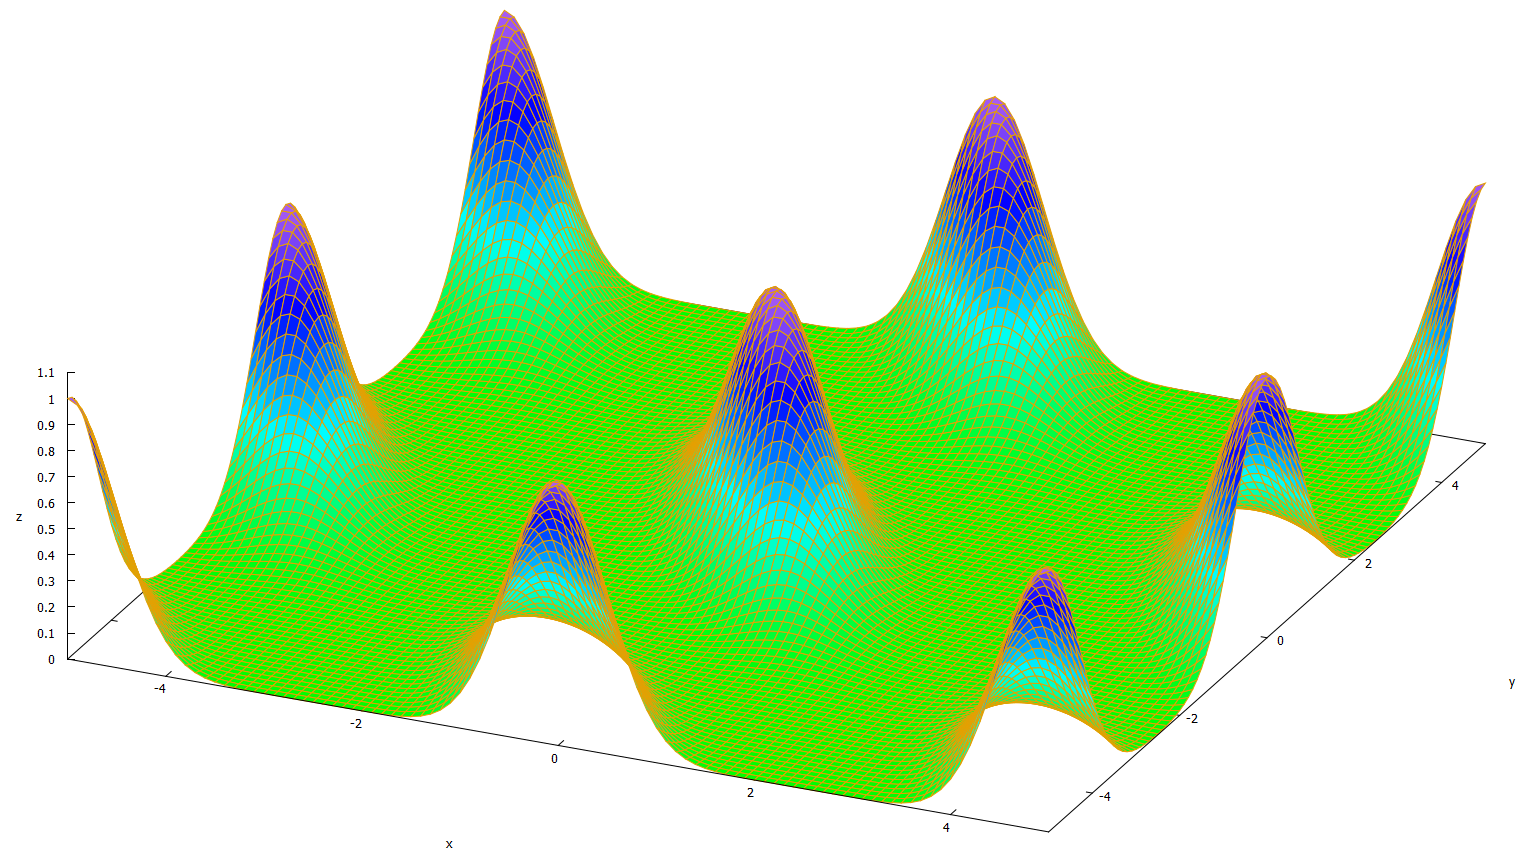
\includegraphics[width=\textwidth]{repeated_gaussians.png}
\caption{Inverse fourier transform of $D_{L, r}$, the ``repeated gaussians''}
\label{repeated_gaussians}
\end{figure}
Therefore, we can approximate the discrete gaussians on $L$ by applying the discrete fourier transformation on an approximation of this source distribution. Classically, this is of no use as we require exponentially many points to represent the source distribution well enough. However, the quantum fourier transform allows us to process exponentially many points in polynomial time, given a suitable superposition of them, something like
\begin{equation}
\sum_{x \in \R^n} e^{-\mathrm{dist}(x, L)^2} |x\rangle \nonumber
\end{equation}
Of course, we cannot sum over $\R$. In reality, we will use all points on a fine grid within the fundamental parallelepiped. Creating this state is not easy however, due to a caveat inherent to quantum computation. The first step of the ``sample lattice points and add noise'' still works, leading to a state that looks like
\begin{equation}
\sum_{x \in \R^n} e^{-\|x - \kappa(x) \|^2} |x\rangle \otimes |\kappa(x)\rangle \nonumber
\end{equation}
There is one problem in this equation though. The qbits containing the noisy point $|x\rangle$ are entangled with the original lattice point we added the noise to, namely $|\kappa(x)\rangle$. In quantum mechanics, all operations have to be reversible, so we cannot just ``drop'' the unwanted qbits without destroying the superposition we need. But since we can compute $|\kappa(x)\rangle$ from $|x\rangle$ using the BDD-oracle, we can ``uncompute'' the $|\kappa(x)\rangle$ part by applying the quantum gates of the oracle in reverse  and get the required superposition.

\paragraph{Details}
Let  $d =\alpha q/ r\sqrt{2n}$ and $R = 2^{3n}d\lambda_n(L^*)\sqrt{n}$ be a big enough integer (representing the fine grid size). Then we claim that the effect of the QFT can be described by
\begin{equation}
\QFT \sum_{x \in \frac 1 R L^*} \rho_d(x) \left|x \mod \mathcal{P}(B^*)\right\rangle = \det(RB) \sum_{t \in L} \rho_{1/d}(t) \left|t \mod \mathcal{P}(RB)\right\rangle \label{eq_result_qft}
\end{equation}
where $\mathcal{P}(B)$ is the fundamental parallelepiped generated by the basis vectors in $B$. When we consider the limit $R \to \infty$, this corresponds to the abstract idea presented earlier, as the left part becomes an integral and the $t \mod \mathcal{P}(RB)$ becomes $t$. We have
\begin{equation}
\begin{split}
&\QFT \sum_{x \in \frac 1 R L^*} \rho_d(x) \left|x \mod \mathcal{P}(B^*)\right\rangle \\
=& \ \QFT \sum_{x \in \frac 1 R L^* \cap \mathcal{P}(B^*)} \rho_d(x + L^*) \left|x\right\rangle \\
=& \ \sum_{t \in L \cap \mathcal{P}(RB)} \ \sum_{x \in \frac 1 R L^* \cap \mathcal{P}(B^*)} \exp(-2\pi i \langle x, t \rangle) \rho_d(x + L^*) \left|t\right\rangle \\
=& \ \sum_{t \in L \cap \mathcal{P}(RB)} \ \sum_{x \in \frac 1 R L^*} \exp(-2\pi i \langle x, t \rangle) \rho_d(x) \left|t\right\rangle \\
=& \det(RB)  \sum_{t \in L \cap \mathcal{P}(RB)} \ \sum_{x \in RL} \rho_{1/d}(x - t) \left|t\right\rangle \\
=& \det(RB) \sum_{t \in L} \rho_{1/d}(t) \left|t \mod \mathcal{P}(RB)\right\rangle \nonumber
\end{split}
\end{equation}
where the second-last line holds due to the Poisson summation formula (Since $\rho$ is equal to its fourier transformation, so $\rho_d = \hat\rho_{1/d}$). Here the use of the QFT on lattices should be the natural extension from the QFT on the coefficients, i.e.
\begin{equation}
\begin{split}
&\QFT \sum_{x \in \frac 1 R L \cap \mathcal{P}(B)} f(x) \left|x\right\rangle = \QFT \sum_{z \in \Z_R^n} f\left(\frac {Bz} R \right) \left|\frac {Bz} R \right\rangle \\
:=& \sum_{k \in \Z_R^n} \ \sum_{z \in \Z_R^n} f\left(\frac {Bz} R \right) \exp\left(-2\pi i\frac {\langle k, z \rangle} R\right) \left|B^* k\right\rangle \\
=& \sum_{k \in \Z_R^n} \ \sum_{x \in \frac 1 R L \cap \mathcal{P}(B)} f(x) \exp\left(-2\pi i \langle k, B^{-1}x \rangle \right) \left|B^* k\right\rangle \\
=& \sum_{k \in \Z_R^n} \ \sum_{x \in \frac 1 R L \cap \mathcal{P}(B)} f(x) \exp\left(-2\pi i \langle B^*k, x \rangle \right) \left|B^* k\right\rangle \\
=& \sum_{y \in L^* \cap \mathcal{P}(RB^*) } \ \sum_{x \in \frac 1 R L \cap \mathcal{P}(B)} f(x) \exp\left(-2\pi i \langle y, x \rangle \right) \left|y\right\rangle \nonumber
\end{split}
\end{equation}
This transform can be done by a quantum computer in polynomial time by multiplying the input register with $RB^{-1}$, then applying the standard QFT and then multiplying the result with $B^*$.

Note that the second term in the QFT result shown above (equation \ref{eq_result_qft}) is almost exactly what we want: When we measure this state, we get $t \mod \mathcal{P}(RB)$ for a $t$ chosen from $D_{L, 1/d\sqrt{2}}$ (since the probability of getting $t$ is proportional to $\rho_{1/d}(t)^2 = \rho_{1/d\sqrt{2}}(t)$). By the following lemma, we can efficiently get $t$ from $t \mod \mathcal{P}(RB)$, and therefore get a sample from $D_{L, 1/d\sqrt{2}} = D_{L, r\sqrt{n}/\alpha q}$. 

We can use the lemma, since $\lambda_1(RL) = R\lambda_1(L) \geq 2^{3n}d\sqrt{n}$ by using $\lambda_n(L^*)\lambda_1(L) \geq 1$ (by \ref{gaussian_length_bound}). In particular, $\lambda_1(RL) \geq d\sqrt{2n}$ and solving $\mathrm{BDD}_{RL, d\sqrt{n}/\sqrt{2}}$ is equivalent to solving $\mathrm{BDD}_{L, d\sqrt{n}/R\sqrt{2}}$ which is possible in polynomial time because $d\sqrt{n}/R\sqrt{2}$ is exponentially small (e.g. by using Babai's nearest plane algorithm).

\paragraph{Lemma 2}
Let $L = \mathcal{L}(B)$ be a lattice, $c > 0$ and $x \sim D_{L/c, \gamma}$ be a random variable with $\lambda_1(L) \geq 2\gamma\sqrt{n}$ and define $x' := x \mod \mathcal{P}(B)$. Assume we have access to an oracle for $\mathrm{BDD}_{L, \gamma\sqrt{n}}$. Then we can efficiently calculate $x$ given $x' = x \mod \mathcal{P}(B)$ with probability of at least $1 - 2^{-2n}$.

\begin{proof}
By \ref{gaussian_length_bound}, the probability that $\|x\| < \gamma\sqrt{n}$ is at least $1 - 2^{-2n}$. If this is the case, we have that $\| x - \kappa(x) \| < \gamma\sqrt{n}$, and so $\|\kappa(x') - x'\| < \gamma\sqrt{n}$. By using the oracle, we can calculate $\kappa(x')$.

Now we use that $\lambda_1(L) \geq 2\gamma\sqrt{n}$. This yields that $\kappa(x) = 0$, since the distance between the lattice points $0$ and $\kappa(x)$ is $< 2\gamma\sqrt{n} \leq \lambda_1(L)$. Similarly, we have $\kappa(x) - \kappa(x') = x - x'$, because the distance between the lattice points  $\kappa(x) - \kappa(x')$ and $x - x'$ is
\begin{equation}
\| \kappa(x) - \kappa(x') - x + x' \| \leq \| \kappa(x) - x \| + \| \kappa(x') - x' \| < 2\gamma\sqrt{n} \leq \lambda_1(L) \nonumber
\end{equation}
Therefore we find $x$ by $x = x' + \kappa(x) - \kappa(x') = x' - \kappa(x')$.

The intuition in this argument is that $x$ is distributed very narrowly around the origin. Therefore, $x \mod \mathcal{P}(B)$ is very close to one of the corners of the fundamental parallelepiped, and the location of $x \mod \mathcal{P}(RB)$ relative to this corner is the location of $x$ relative to the origin. \qedhere
\end{proof}

\paragraph{Creating the initial state} 
We have shown that we can get a sample from the right side of equation \ref{eq_result_qft}, so it remains to be shown that we can efficiently create the state on the left side, namely
\begin{equation}
\sum_{x \in \frac 1 R L^*} \rho_d(x) |x \mod \mathcal{P}(B^*)\rangle \nonumber
\end{equation}
It is not obvious, but this state corresponds to the ``repeated gaussian'' distribution mentioned earlier: Taking the gaussian (almost continous for large $R$) modulo the fundamental parallelepiped yields a distribution in which there are ``hills'' in each corner of the parallelepiped, and by filling the complete space with copies of the parallelepiped, we get the ``repeated gaussian'' distribution.

By dividing the register by $R$, we can easily get this state when we start with the state
\begin{equation}
\sum_{x \in L^*} \rho_{Rd}(x) |x \mod \mathcal{P}(RB^*)\rangle \nonumber
\end{equation}
As shown in \cite{Reg} 3.2, we can efficiently create the state
\begin{equation}
\sum_{x \in L^*} \rho_{Rd}(x) |x\rangle \nonumber
\end{equation}
Classically, it looks like we could just take this state modulo $\mathcal{P}(RB^*)$ and be done. The problem is that quantum operations have to be reversible, so we have to be able to calculate $x$ from $x \mod \mathcal{P}(RB^*)$ in order to do this. Luckily, we can do that using Lemma 2:

We have $\lambda_1(RL^*) = R\lambda_1(L^*) \geq 2Rd\sqrt{n}$ since
\begin{equation}
2d\sqrt{n} = \frac {\alpha q} {r \sqrt{2}} \leq \frac {\alpha q} {2q\eta_\epsilon(L)} = \frac \alpha {2\eta_\epsilon(L)} \leq \frac 1 {2\eta_\epsilon(L)} \leq \frac {\lambda_1(L)} 2 \nonumber
\end{equation}
where the last inequality follows from \ref{smoothing_parameter_lower_bound} and we can solve $\mathrm{BDD}_{RL^*, Rd\sqrt{n}}$ which is equivalent to $\mathrm{BDD}_{L^*, d\sqrt{n}} = \mathrm{BDD}_{L^*, \alpha q/r\sqrt{2}}$ by using the oracle constructed earlier. \qedhere
\end{proof}

\paragraph{Proof of \ref{hardness_lwe}}
The idea is to start with samples of a very wide gaussian distribution which are easy to generate, and then improve them using the lemma \ref{recursive_step} above. This way, we can get samples of a very narrow gaussian distribution. Among $n^2$ of these are $n$ linearly independent one with very high probability, so we can use them to solve SIVP.

\subparagraph{Show} For a given $r \geq n \sqrt{2}\lambda_n(L)/\alpha$ we can efficiently sample from $D_{L, r}$. \\
As shown in \cite{Reg}, we can efficiently sample from $D_{L, r'}$ for some computable, exponentially large $2^{3n}\lambda_n(L) \geq r' \geq 2^{2n} \lambda_n(L)$. The idea in that argument is to use a LLL basis of $L$. Let $\epsilon = 2^{-n}$ and apply lemma \ref{recursive_step} repeatedly on these samples to create shorter ones. The condition of \ref{recursive_step} is fullfilled as long as the input radius is $\geq q \sqrt{2n} \lambda_n(L)$, because by \ref{smoothing_parameter_upper_bound} and \ref{lambda_dual_lattice} we have
\begin{equation}
\sqrt{2}q\eta_\epsilon(L) \leq \frac {q \sqrt{2n}} {\lambda_1(L^*)} \leq q \sqrt{2n} \lambda_n(L) \nonumber
\end{equation}
Therefore we can reach the given $r$ by repeated applications, because we have by assumption that $r \geq n\sqrt{2}\lambda_n(L)/\alpha \geq q \sqrt{2n} \lambda_n(L) \sqrt{n}/\alpha q$.
Since every application of the recursive step shrinks the radius by a factor of $2$, we can get samples of $D_{L, r}$ through polynomially many repetitions (as $\log r'/r$ is polynomial in $n$).

\paragraph{Lemma 3} The probability that $n^2$ independent samples of $D_{L, r}$ for some $r \geq \sqrt{2}\eta_\epsilon(L)$ are contained in any $n-1$ dimensional hyperplane is exponentially small. In other words, the probability that there are $n$ linearly independent samples among those $n^2$ ones is exponentially close to $1$.

\begin{proof} \noqed
See \cite[3.16]{Reg}.
\end{proof}

Now it looks like we could just get $n^2$ samples from $D_{L, r}$ for $r = n\sqrt{2}\lambda_n(L)/\alpha$ and output $n$ linearly independent ones from among them (they have length $\leq 2n\sqrt{n}\lambda_n(L)/\alpha$ by \ref{gaussian_length_bound}). The only problem however is that we do not know $\lambda_n(L)$, so we cannot give the right $r$ to the sampling oracle. We can however apply the whole procedure for each $r_k = 2^{-k}r' n\sqrt{2}/\alpha$ where $r'$ is the exponential upper bound for $\lambda_n(L)$ mentioned above and take the shortest set of independent samples we find. Since $2^{3n}\lambda_n(L) \geq r' \geq 2^{2n} \lambda_n(L)$, there must be some $k \in \{ 2n, ..., 3n \}$ so that 
\begin{equation}
r_k = 2^{-k} r' n\sqrt{2}/\alpha \in \left[n \sqrt{2}\lambda_n(L)/\alpha, 2n \sqrt{2}\lambda_n(L)/\alpha \right] \nonumber
\end{equation}
So when we try that $k$, we sample $n^2$ vectors from $D_{L, r_k}$ and find $n$ linearly independent vectors of length $\leq 2n \sqrt{2n}\lambda_n(L)/\alpha$ with high probability, which solves $\mathrm{SIVP}_{2n\sqrt{2n}/\alpha}$. \qedhere
\end{proof}












\remark[A cryptosystem]
\label{lwe_cryptosystem}
Consider the following cryptosystem. While there are easier schemes based on LWE, this one is the most efficient one and will become important later as basis for Crystals Kyber.
\begin{description}
\item[Secret Key] Choose uniform $s \sim \Psi_\alpha$
\item[Public Key] Choose $s, e_1 \sim \Psi_\alpha^n$ and $A \in \Z_q^{n \times n}$ uniformly, publish $(A, b) = (A, s^TA + e_1^T)$
\item[Encryption] Choose $r, e_2 \sim \Psi_\alpha^n, e_3 \sim \Psi_\alpha$, encrypt $m \in \{ 0, 1 \}$ as $(Ar + e_2, br + e_3 + \lfloor \frac q 2 \rceil m)$
\item[Decryption] On receiving $(u, v)$, check if $v - s^Tu$ is closer to $0$ or $\lfloor \frac q 2 \rceil$
\end{description}
When $2\sqrt{n}/q \leq \alpha \leq 1/3\sqrt{qn}$, then this scheme is both correct and secure under the assumption that SIVP for polynomial approximation factors is worst case quantum hard. A possible choice of parameters would therefore be $q = 36n^2$ and $\alpha = 1/18n\sqrt{n}$.

\paragraph{Correctness}
\begin{proof}
Let $s, r, e_1, e_2 \sim \Psi_\alpha^n, e_3 \sim \Psi_\alpha, A \sim \Z_q^{n \times n}$ and $x \sim \{ 0, 1 \}^n$ be random variables representing the values chosen by the procedure, and let $b := s^TA + e_1^T$. Then the input to the decryption procedure is $(u, v)$ with $u = Ar$ and $v = br + e_3 + \lfloor \frac q 2 \rceil m$. Therefore, we get
\begin{equation}
v - s^Tu = s^TAr + e_1^Tr + e_3 + \left\lfloor \frac q 2 \right\rceil m - s^TAr =  e_1^Tr + e_3 + \left\lfloor \frac q 2 \right\rceil m\nonumber
\end{equation}
With high probability, we have that $\| e_1^T \|, \| r \| \leq \alpha q \sqrt{n}$. By Cauchy-Schwarz, we have that $| e_1^Tr + e_3 | \leq \alpha^2 q^2 n + \alpha q = \alpha q (\alpha q n + 1)$. Since $\alpha \leq 1/3\sqrt{nq}$, it follows that for $\sqrt{qn} \geq 3$, we have
\begin{equation}
| e_1^Tr + e_3 | \leq \frac {\sqrt{q}} {3\sqrt{n}} ( \sqrt{qn}/3 + 1 ) = \frac q 9 + \frac {q} {3\sqrt{nq}} \leq \frac {2q} 9 < \frac q 4 \nonumber
\end{equation}
Therefore, the distance between $v - u^Ts$ and $m\lfloor \frac q 2 \rceil$ is at most $\frac q 4$, and so we have that $m = 0$ if $v - s^Tu$ is closer to $0$, and $m = 1$ if $v - s^Tu$ is closer to $\lfloor \frac q 2 \rceil$, which proves correctness. \qedhere
\end{proof}

\paragraph{Security}
\begin{proof}
Using the reductions \ref{decision_to_search}, \ref{secret_error_distribution}, \ref{average_to_worst} and \ref{hardness_lwe} and assuming the quantum hardness of SIVP for the polynomial approximation factor $2n\sqrt{2n}/\alpha$, we get that an adversary cannot distinguish between $A_{s, \Psi_\alpha}$ for $s \sim \Psi_\alpha$ and $(A, u)$ for uniform $A, u$.
\subparagraph{Show} An adversary cannot distinguish between encryptions of $0$ and encryptions of $1$. For this, we use that computational indistinguishability is transitive with respect to polynomial chaining. For independent and uniformly distributed random variables $U_1, U_2$ it holds that
\begin{equation}
\begin{split}
&\left(A, As + e_1, Ar + e_2, s^TAr + e_1^Tr + e_3 \right) \\
\text{ind. from } & \left(A, U_1, Ar + e_2, U_2 \right) \\
\text{ind. from } & \left(A, As + e_1, Ar + e_2, U_2 \right) \\
\text{ind. from } & \left(A, As + e_1, Ar + e_2, U_2 + \left\lfloor \frac q 2 \right\rceil \right) \\
\text{ind. from } & \left(A, U_1, Ar + e_2, U_2 + \left\lfloor \frac q 2 \right\rceil \right) \\
\text{ind. from } & \left(A, As + e_1, Ar + e_2, s^TAr + e_1^Tr + e_3 + \left\lfloor \frac q 2 \right\rceil \right)
\end{split} \nonumber
\end{equation}
To see that the first and last indistinguishability hold, assume that an adversary could distinguish between both distributions. Then, given samples of $(A, b)$ with either $b \sim A_{s, \Psi_\alpha}$ or $b$ uniform, he could choose $r, e_2 \sim \Psi_\alpha^n, e_3 \sim \Psi_\alpha$ and call the oracle with $(A, b, Ar + e_2, br + e_3)$. If $(A, b) \sim A_{s, \Psi_\alpha}$, then $(A, b, Ar + e_2, br + e_3)$ is distributed identically to $(A, As + e_1, Ar + e_2, s^TAr + e_1^Tr + e_3)$ and if $b$ is uniform, then $(A, b, Ar + e_2, br + e_3)$ is distributed identically to $(A, U_1, Ar + e_2, U_2)$. Therefore, the adversary could solve decision LWE, a contradiction.

Since the first distribution is equal to an encryption of $0$ and the last one is equal to an encryption of $1$, we see that an adversary cannot distinguish between them, so the scheme is secure. \qedhere
\end{proof}

\remark[Choice of parameters]
As a summary of the results of this section, we will list the conditions the LWE parameters must satisfy so that we get the corresponding security guarantees. Note that in some cases, other values may not lead to an insecure system, we just cannot prove its security the same way we did in this section:
\begin{itemize}
\item $q$ must be a prime. This was never mentioned explicitly, but it is the reason that $\langle x, a \rangle$ for a constant $a \neq 0$ and a uniform $x$ is uniform on $\Z_q$, which we used multiple times.
\item $\alpha q \geq 2\sqrt{n}$ so that \ref{hardness_lwe} applies.
\item The error must not be too big so that the LWE structure is still recognizable. As in \ref{unique_lwe_solution}, is suffices if $\alpha \leq \frac 1 {2\sqrt{n}} - \epsilon$.
\item There must be enough samples so that there is a unique solution. When $s$ is uniformly chosen, then, as in \ref{unique_lwe_solution}, it is sufficient if $\omega(n\log q)$ or $\Omega(n\log q)$ if $\alpha \in o(1)$. However, by drawing the secret from the error distribution (as in \ref{secret_error_distribution}) and only accepting short secrets, a calculation as in \ref{unique_lwe_solution} shows that $\Omega(n)$ samples are sufficient.
\end{itemize}
A possible cryptographic scheme is presented in \ref{lwe_cryptosystem} (tighter bounds on the error are required for this scheme). The key sizes we have there are usual for cryptosystems based on LWE:
\begin{itemize}
\item Private key size is $\Theta(n)$ elements of $\Z_q$
\item Public key size is $\Theta(n^2)$ elements of $\Z_q$
\item Ciphertext size is $\Theta(n)$ elements of $\Z_q$
\end{itemize}
The quadratic public key size is still not competitive compared to schemes based on other popular problems. However, we will now see how to decrease this key size further, under slightly stronger security assumptions.

% IDEAL LATTICES AND RLWE

\chapter{Ideal lattices and Ring LWE}

\motivation
Standard LWE can be used to build cryptosystems with practical relevance, like for example in the second round NIST candidate FrodoKEM (\cite{FrodoKEM}). However, the quadratic key sizes and processing time are not as efficient as one can achieve by using other approaches. This can be fixed by introducing additional structure to the lattices. The most widespread idea is to switch to so called anticyclic lattices, where for each lattice point $(x_1, ..., x_n)$ the anticyclic rotation $(x_2, ..., x_n, -x_1)$ is also a lattice point. Of course, this requires stronger security assumption (i.e.\ that the problems are even hard if restricted to lattices with the certain property), but using the corresponding variant of LWE, called Ring Learning with Errors, leads to schemes with only linear key sizes and quasilinear runtime. In this section, we will show how this can be done, and we will also see an algebraic generalization of the anticyclic lattices, the so-called ideal lattices.

\remark[Ideals are lattices]
Let $\mathcal{O}_K$ be the ring of integers in a number field $K = \mathbb{Q}(\alpha)$. Then a fractional ideal $I \leq \mathcal{O}_K$ is a free $\Z$-module of rank $n = [K : \mathbb{Q}]$ as shown for example in \cite[2.10]{Neukirch}. Therefore, $I$ is $\Z$-module isomorphic to $\Z^n$, so we can identify $I$ with a lattice in $\R^n$. However, the additive structure of any lattice is always $\Z^n$, so this is quite boring. Lattices only become interesting when we introduce a norm. So when we work with ideals as lattices, the concrete identification of ideals $I$ with lattices in $\R^n$ matters, as this induces a norm on $K$ resp. $I$.

\remark[Embeddings and the norm]
$K$ is a $\mathbb{Q}$-vector space of dimension $n = [K : \mathbb{Q}]$, so we can find vector space embeddings (injective homomorphisms) $\sigma: K \to \R^n$ with $\sigma(\mathcal{O}_K)$ is a lattice in $\R$. Then also $\sigma(I)$ is a lattice for a fractional ideal $I \leq \mathcal{O}_K$, and lattices of this form are called ideal lattices. Therefore, ideal lattices are special in so far that they have a product induced by the multiplication in $K$, even though this can be quite well hidden by the transformation through $\sigma$.

One obvious way to choose $\sigma$, which we will call the ``naive embedding'', is to choose the coefficients in the basis representation of a value, i.e.
\begin{equation}
\sigma': K \to \R^n, \quad \sum_{i = 0}^{n - 1} a_i \alpha^i \mapsto (a_i)_i \nonumber
\end{equation}

\cite{LyuPeiReg} have used another embedding, the canonical embedding from algebraic number theory. Since a number field $K$ is separable, there are exactly $n$ $\mathbb{Q}$-field homomorphisms $\tau: K \to \mathbb{C}$. These homomorphisms are either real (i.e.\ $\tau(K) \subseteq \R$) or complex. The complex homomorphisms come in pairs $\tau, \overline{\tau}$, where $\overline{\tau} = \overline{\cdot} \circ \tau$ is the complex conjugate of $\tau$. Let the number of real homomorphisms be $s_1$ and the number of pairs of complex homomorphisms be $s_2$. Then can define the canonical embedding
\begin{equation}
\sigma: K \to K_{\R} \cong \R^{s_1 + 2s_2}, \quad \alpha \mapsto (\tau(\alpha))_\tau \nonumber
\end{equation}
where $K_\R$ is the Minkowski-Space, that can be characterized as
\begin{equation}
K_\R := \left\{ x \in \mathbb{C}^{\mathrm{Hom}_{\mathbb{Q}}(K, \mathbb{C})} | x_\rho \in \R, x_{\overline{\tau}} = \overline{x_\tau} \right\} \nonumber
\end{equation}
where $\rho$ runs through the real homomorphisms and $\tau$ runs through the complex ones. For more information on Minkowski theory, see e.g. \cite{Neukirch}. On $K_\R$, we have the inner product $\langle \cdot, \cdot \rangle$ from $\mathbb{C}^n$, which induces a norm on $K$ and we can transfer this norm on $\R^{s_1 + 2s_2}$ by using an orthonormal basis. A nice property of this embedding is that for $x, y \in K$ we have $\sigma(xy) = \sigma(x)\sigma(y)$, where the second product is component-wise. In particular, we get that $\| x y \| \leq \| x \| \| y \|$. Using this embedding, \cite{LyuPeiReg} have shown the results from this section in a more general context (for arbitrary cyclotomic number fields). We however will focus on the case of cyclotomic number fields of a power-of-two degree, as this is most relevant for cryptographic applications.

\definition
For this whole section, let $n$ be a power of two, $f = \Psi_n = X^n + 1$ be the $2n$-th cyclotomic polynomial and $K = \mathbb{Q}[\zeta] \cong \mathbb{Q}[X]/(f)$ be the corresponding number field with ring of integers $\mathcal{O}_K$, where $\zeta = \exp(\pi i / n)$ is a $2n$-th root of unity.
\\\\
One reason why this is an important special case is the following result that shows that both previously discussed embeddings lead to the same norm on $K$ (except for a fixed factor $\sqrt{n}$).

\proposition{Equivalence of ideal lattice norms}
\label{equivalence_norms}
For $\alpha = \sum c_i \alpha^i \in K$, we have that $\sqrt{n} \| \sigma'(\alpha) \| = \sqrt{n} \| (c_i)_i \| = \| \sigma(\alpha) \|$ where 
\begin{equation}
\sigma': K \to \R^n, \quad \sum_{i = 0}^{n - 1} c_i \zeta^i \mapsto (c_i)_i \nonumber
\end{equation}
is the ``naive embedding'' and
\begin{equation}
\sigma: K \to K_{\R}, \quad \zeta \mapsto (\tau(\zeta))_\tau \nonumber
\end{equation}
is the canonical embedding.

Because of this result, we sometimes will not distinguish between the concrete norms.

\begin{proof}
Let $\tau_1, ..., \tau_n \in \mathrm{Aut}_{\mathbb{Q}}(K)$ be the $\mathbb{Q}$-Automorphisms of $K$. By using $K \subseteq \mathbb{C}$, they are also exactly the $\mathbb{Q}$-embeddings of $K$. Consider the transformation 
\begin{equation}
f: \mathbb{C}^n \to \mathbb{C}^n, \quad (c_i)_i \mapsto \frac 1 {\sqrt{n}} (\sigma_i\left(\sum_{i = 0}^{n - 1} c_i \zeta^i \right))_i \nonumber
\end{equation}
We have to show that $f$ is an isometry, since by identifying $K_\R$ with a subset of $\mathbb{C}^n$, we obviously have that 
\begin{equation}
f\big|_{\sigma'(K)} = \sigma \circ \sigma'\big|_{\sigma'(K)}^{-1} \nonumber
\end{equation}
Define the matrix $A = (a_{ij}) \in \mathbb{C}^{n \times n}$ by $a_{ij} = \frac 1 {\sqrt{n}} \sigma_i(\zeta^j)$. Then $f$ is linear and represented by the matrix $A$, so $f(x) = Ax$ because
\begin{equation}
f(c)_j = \frac 1 {\sqrt{n}} \sigma_j\left(\sum_i c_i \zeta^i\right) = \frac 1 {\sqrt{n}} \sum_i c_i \sigma_j(\zeta^i) = \sum_i c_i a_{ij} = (Ac)_j \nonumber
\end{equation}
On the other hand, it holds that the $i, j$-th entry of $A^\dagger A$ is
\begin{equation}
\begin{split}
&\sum_{k = 0}^{n - 1} \overline{a_{ki}} a_{kj} = \frac 1 n \sum_{k = 0}^{n - 1} \overline{\sigma_k(\zeta^i)} \sigma(\zeta^j) = \frac 1 n \sum_{k = 0}^{n - 1} \sigma_k(\zeta^{-i}) \sigma(\zeta^j) \\
=& \frac 1 n \sum_{k = 0}^{n - 1} \sigma_k(\zeta^{j - i}) = \frac 1 n \mathrm{Tr}(\zeta^{i-j})
\end{split} \nonumber
\end{equation}
And since $\mathrm{Tr}(\zeta^i) = 0$ if $i \neq 0$ and $\mathrm{Tr}(\zeta^i) = n$ if $i = 0$, we get that $A^\dagger A = I$ and so $f$ is a linear isometry.\qedhere
\end{proof}

\definition[Algebraic structures]
For the definition of Ring LWE and the results, we have to consider some algebraic structures:
\begin{itemize}
\item Define the ring $R = \mathcal{O}_K = \Z[\zeta]$ and $R_q = R / qR = \Z_q[\zeta]$.
\item Have the Minkowski-Space (it is a ring) $K_\R$ with the ring-embedding $\sigma: K \to K_\R$ as above.
\item Define the $\Z$-module $\T_q := K_\R / \sigma(qR)$ with a norm-like operation as in \ref{lattice_norm}, i.e.\ for $x \in \T_q$ have $\| t \| := \min \{ \| x \| | x \in \R[X] / (f), t = x \mod qR \}$ the norm of the shortest representative in $K_\R$.
\item Have the $R$-module $K / qR$, which embeds into $\T_q$ by taking $\sigma: K \to K_\R$ ``mod $q$''
\begin{equation}
\sigma: K / qR \to K_\R / \sigma(qR), \quad [x] \mapsto [\sigma(x)] \nonumber
\end{equation}
This $\sigma$ is a $R$-module homomorphism. We also use the norm on $K / qR$ induced by this embedding $\sigma$. We also embed the ring $R_q$ into $K / qR$, and use the induced norm on $R_q$.
\item For a fractional ideal $I$ of $R$ have the $R$-modules $I / qI$ and $I^{-1} / qI^{-1}$. Also have the multiplication 
\begin{equation}
I / qI \times I^{-1} / qI^{-1} \to R_q, \quad ([x], [y]) \mapsto [xy] \nonumber
\end{equation}
\item For a fractional ideal $I$, also define the ``dual'' ideal $I^\vee := \{ x \in R | \mathrm{Tr}(x\bar{I}) \subseteq \Z \}$ whose image under $\sigma$ is the dual lattice $\sigma(I)^*$, since $\langle \sigma(x), \sigma(y) \rangle = \mathrm{Tr}(x\bar{y})$. We have $I^\vee = R^\vee I^{-1}$, and $R^\vee$ is also called the codifferent ideal. If $n$ is a power of two, we have that $R^\vee = \frac 1 n R$, so we will no go into the properties of $I^\vee$ in detail (for arbitrary cyclotomic number fields, this is important, see \cite{LyuPeiReg}).
\end{itemize}

\definition[Ring LWE]
Analogue to normal LWE, we define a discrete and a continuous version of Ring LWE:
\paragraph{Continuous} For a probability distribution $\chi$ on $\T_q$, we define the Ring LWE distribution $A_{s, \chi}$ as the probability distribution that results from choosing an $a \in R_q$ uniformly, $e \sim \chi$ independently and outputting $(a, \sigma(as) + e)$.
\paragraph{Discrete} For a probability distribution $\chi$ on $R_q$, we define the $A_{s, \chi}$ as the distribution that results from choosing an $a \in R_q$ uniformly, $e \sim \chi$ independently and outputting $(a, as + e)$.
\\\\
Then the (average case) Ring Learning with Errors problem $\mathrm{RLWE}_{q, \chi}$ is: For a uniformly chosen $s \in R_q$, given samples from $A_{s, \chi}$, find $s$.

\remark[RLWE Error]
\label{rlwe_error}
In the case of LWE, usually we used $\Psi_\alpha$ as the error distribution. In RLWE, this would correspond to an error $e = \sum e_i \zeta^i \in \T_q$ where $e_0, ..., e_{n - 1} \sim \Psi_\alpha$ are iid.. However, the hardness proof \ref{hardness_lwe} does not work with this distribution, since this distribution is not closed with respect to multiplication with a constant element in $K$. Instead, we need elliptical gaussian distributions. For $\alpha \in \R^n, \alpha \geq 0$ define the elliptical gaussian distribution $\nu_\alpha$ on $K_\R$ with results from choosing each component $e_\tau \sim \nu_{\alpha_i}$.

Then we have that for $e \sim \nu_\alpha$ and $x \in K$, the product $\sigma(x)e$ is distributed according to $\nu_{\alpha \sigma(x)}$ (using component-wise multiplication) since the canonical embedding transforms multiplication in $K$ to component-wise multiplication in $K_\R$. In particular, if $\alpha_i \leq c$ for all $i$ with $c > 0$, then $(\alpha \sigma(x))_i \leq c\sigma(x)_i \leq c \| \sigma(x) \|_\infty$. We still write $\nu_s$ for $s > 0$ when we mean the distribution $\nu_{(s)_i}$ on $R$ with the error vector $(s)_i \in \R^n$.

\paragraph{Continuous Error} We now can use this distribution modulo $q$ as RLWE error, i.e.\ define $\Psi_\alpha$ on $\T_q$ as the probability distribution you get from sampling from $\nu_{q\alpha}$ and taking the result $\mod \sigma(qR)$.

\paragraph{Discrete Error} For the discrete variant of RLWE, we also need a discrete error distribution on $R_q$. Define $\bar{\Psi}_\alpha$ as the probability distribution that results from sampling $e \sim \nu_{q \alpha}$ and outputting $\sigma^{-1}(\lfloor e \rceil) \mod qR$, where we round $e \in K_\R$ by $\lfloor e \rceil = \kappa_{\sigma(R)}(e)$. Usually, calculating $\kappa_L(x)$ is hard, but in the case $L = \sigma(R)$, it can be done efficiently:

We can extend $\sigma: \mathbb{Q}[X] / (f) = K \to K_\R$ to the ring homomorphism
\begin{equation}
\sigma: \R[X] / (f) \to K_\R, \quad \left[ \sum a_i X^i \right] \mapsto \left( \sum a_i \zeta^{ik} \right)_{\tau_k} \nonumber
\end{equation}
with a root of unity $\zeta = \exp(\pi i / n) \in \mathbb{C}$ and the field embeddings $\tau_k \in \mathrm{Hom}_{\mathbb{Q}}(K, \mathbb{C})$ with $\tau(\zeta) = \zeta^k$. This extension is bijective, as a polynomial of degree $< n$ is unique characterized by its value at $n$ different points. As shown in \ref{equivalence_norms}, the ``naive'' norm on $\R[X] / (f)$ is (up to a factor) equal to the norm on $K_\R$, so using that extension, we have that $\kappa_{\sigma(R)}(x) = \sigma(\kappa_R(\sigma^{-1}(x)))$. We can easily calculate $\kappa_R(y)$ by rounding each of the coefficients in the linear combination $y = [\sum a_i X^i] \in \R[X] / (f)$.

\lemma
\label{rounding_kr_commutes}
Let $\tau: K \to K$ be a $\mathbb{Q}$-automorphism of $K$. We have that $\sigma \circ \tau \circ \sigma^{-1} = \restr{\pi_\tau}{\sigma(K)}$ where $\pi_\tau$ is a permutation of the vector components in $K_\R$ as
\begin{equation}
\pi_\tau: K_\R \to K_\R, \quad (x_\rho)_\rho \mapsto (x_{\rho \circ \tau})_\rho \nonumber
\end{equation}
Furthermore, for $e \in K_\R$ it holds that $\pi_\tau(\lfloor e \rceil) = \lfloor \pi_\tau(e) \rceil \in \sigma(R)$.

\begin{proof}
For $x \in K$ and a $\mathbb{Q}$-embedding $\rho: K \to K_\R$, we have
\begin{equation}
(\sigma \circ \tau \circ \sigma^{-1})(\sigma(x))_\rho = \sigma(\tau(x))_\rho = \rho(\tau(x)) = \sigma(x)_{\rho \circ \tau} = \pi_\tau(\sigma(x))_\rho \nonumber
\end{equation}
For $e \in K_\R$, we have
\begin{equation}
\lfloor \pi_\tau(e) \rceil = \kappa_{\sigma(R)}(\pi_\tau(e)) = \pi(\kappa_{\pi_\tau^{-1}(\sigma(R))}(\pi_\tau^{-1}(\pi(e)))) = \pi_\tau(\kappa_{\pi_\tau^{-1}(\sigma(R))}(e)) \nonumber
\end{equation}
since $\pi_\tau$ is an isometry, so $\pi(\kappa_L(x)) = \kappa_{\pi(L)}(\pi(x))$. It is left to show that $\pi_\tau^{-1}(\sigma(R)) = \sigma(R)$, or equivalently that $R = \sigma^{-1}(\pi_\tau(\sigma(R)))$. This holds, since $\tau(R) = R$ and $\sigma \circ \tau \circ \sigma^{-1} = \restr{\pi_\tau}{\sigma(K)}$.\qedhere
\end{proof}

\definition
Also consider a variant of RLWE with unknown, bounded error distributions as we did for LWE. For $\alpha > 0$, define $\mathrm{RLWE}_{q, \leq \alpha}$ as the following problem: For a uniformly chosen $s \in R_q$ and any $\beta \in \R^n, \beta \geq 0$ and $\beta_i \leq \alpha$ for all $i$, find $s$ given samples from $A_{s, \Psi_\beta}$.

\remark[Connection RLWE and LWE]
\label{connection_rlwe_lwe}
Ring LWE can be seen as a special case of LWE, where the samples come in batches. A ring LWE sample $(a, as + e)$ with $a = \sum a_i \zeta^i \in R_q$ and $e \sim \Psi_\alpha$ where $\alpha_1 = ... = \alpha_n = \beta > 0$ with secret $s = \sum s_i \zeta^i \in R_q$ can also be written as
\begin{equation}
\begin{pmatrix} a_0 \\ a_1 \\ \vdots \\ a_{n - 1} \end{pmatrix}
, \
\begin{pmatrix}
a_0 & -a_{n - 1} & -a_{n - 2} & ... & -a_1 \\
a_1 & a_0 & -a_{n - 1} &  & -a_2 \\
\vdots & & & \ddots & \vdots \\
a_{n - 1} & a_{n - 2} & a_{n - 3} & ...& a_0
\end{pmatrix}
\begin{pmatrix} s_0 \\ s_1 \\ \vdots \\ s_{n - 1} \end{pmatrix}
+
\begin{pmatrix} e_0 \\ e_1 \\ \vdots \\ e_{n - 1} \end{pmatrix} 
\nonumber
\end{equation}
by using the the polynomial multiplication
\begin{equation}
as = \sum_{i, j} a_i s_j \zeta^{i + j} = \sum_{i, j} a_i s_j \zeta^{i + j \mod q} = \sum_i \zeta^i \sum_k s_k a_{i - k \mod q} \nonumber
\end{equation}
Since $\sigma$ is a linear isometry and all components of $e$ are independent and distributed according to the same normal distribution, we get that if $e = \sigma\left(\sum e'_i \zeta^i \right)$ all $e'_i$ are iid. and distributed like $\Psi_{\alpha / n}$. Therefore this single RLWE sample is really $n$ LWE samples with all anticyclic rotations of $(a_{n - 1}, ..., a_0)$ as first sample parts. This is also the main reason why RLWE is more efficient than normal LWE: We required a factor of $n$ less samples, so the space and time requirements are significantly lower. It also leads to the following proposition:

\proposition{RLWE to LWE reduction}
\label{rlwe_to_lwe_reduction}
Let $\beta = \frac 1 {n^2} \sum_k \alpha_k$. Then
\begin{equation}
\mathrm{RLWE}_{q, \Psi_\alpha} \leq_p \mathrm{LWE}_{q, \Psi_\beta} \nonumber
\end{equation}

\begin{proof}
Receive RLWE samples $(a = \sum_j a_j \zeta^j, b = \sigma(\sum_j b_j \zeta^j) = \sigma(as) + e)$ and give $(a', b')$ to the oracle where $a' = (a_{n - 1}, ..., a_0)^T$ and $b' = b_0 \in \R / q\Z$. Then $(a', b')$ is a valid LWE sample for secret $s' = (s_0, ..., s_{n - 1})^T$ with $s = \sum_j s_j \zeta^j$, since 
\begin{equation}
as = \sum_{i, j} a_i s_j \zeta^{i + j} = \sum_i \zeta^i \sum_k s_k a_{i - k} = \sum_i \zeta^i \sum_k a'_{k + i} s'_k \nonumber
\end{equation}
so $b_0 = \sum a'_k s'_k + e_0 = \langle a', s' \rangle + e_0$, where we define $a_{j - n} = a_{j + n} = -a_j$ for $j \in \{ 0, ..., n - 1 \}$. Therefore, when the oracle returns $s'$, we return $s = \sum s'_i \zeta^i$.

\subparagraph{The Error} Have $e = \sigma\left(\sum_j e_j \zeta^j\right) \sim \Psi_\alpha$ (extend $\sigma$ to $\sigma: \R/(f) \to K_\R$). Then $e_0, ..., e_{n - 1}$ are gaussian random variables, and
\begin{equation}
\mathrm{Cov}(e_i, e_j) = \frac 1 {n^2} \left(A^\dagger \mathrm{diag}(\alpha) A\right)_{ij} = \frac 1 {n^2} \sum_{k, l} \tau_l\left(\zeta^i\right) \delta_{lk} \alpha_l \overline{\tau_k\left(\zeta^j\right)} = \frac 1 {n^2} \sum_k \tau_k\left(\zeta^{i - j}\right) \alpha_k \nonumber
\end{equation}
by using $A$ and $\tau_0, ..., \tau_{n - 1}$ as in \ref{equivalence_norms}, since $\sigma^{-1}$ is linear and represented by the matrix $\frac 1 n A^\dagger$ in the basis $\zeta^0, ..., \zeta^{n - 1}$. In particular, $\mathrm{Var}(e_0) = \frac 1 {n^2} \sum_k \alpha_k$, so $e_0 \sim \Psi_\beta$. Since $e_1, ..., e_{n - 1}$ are discarded, it does not matter that they might not be independent. \qedhere
\end{proof}

\remark[Unknown to constant error variance reduction]
If the error distribution $\Psi_\beta$ is spherical, i.e.\ $\beta_1 = ... = \beta_n \leq \alpha$ for some $\alpha > 0$, then we can solve Ring LWE for an unknown error distribution $\Psi_\beta$ when given an oracle for $\mathrm{RLWE}_{q, \Psi_\alpha}$ by ``guessing'' the right amount of error we have to add to $\beta$ to be close enough to $\alpha$, as we did in \ref{lwe_leq_alpha_lwe_alpha}. However, if $\Psi_\beta$ is elliptical (i.e.\ $\beta_i \neq \beta_j$ in general), we would have to ``guess'' correctly each component of $\beta$, which is not possible to do in polynomial time. Therefore, the gap between the unknown error variant and the standard RLWE problem is not easy to cross. 

In fact, \cite{LyuPeiReg} could only prove a reduction to a variant of Ring LWE, where the error distribution is unknown, but each component of the error distribution variance is again random and distributed according to the gamma distribution $\Gamma(2, 1)$. This is more like an average-case version of the unknown error distribution RLWE problem, but at least it can be implemented. Additionally, if the number of samples an adversary has access to is fixed, then it is possible to restrict the problem to one fixed, spherical error distribution $\Psi_{(\alpha)_i}$ with slightly larger variance $\alpha > 0$.

\remark
Most hardness results for LWE still hold, namely the average to worst case reduction \ref{average_to_worst}, the reduction to SIVP \ref{hardness_lwe} and that we can draw the secret from the error distribution \ref{secret_error_distribution}. That \ref{average_to_worst} and \ref{secret_error_distribution} still hold is quite easy to see, as we only add and invert the inputs, and $R_q$ is closed under these operations. In the reduction \ref{average_to_worst}, we have to switch to SIVP and BDD on ideal lattices. We will sketch how to modify this reduction so that it works with RLWE.

One important result however, the decision to search reduction \ref{decision_to_search} cannot be adjusted to work with RLWE due to the way we modify the samples. A corresponding result for ideal lattices has been proven by \cite{LyuPeiReg}, and we will present it at the end of this section.

\proposition{SIVP to RLWE reduction}
\label{hardness_rlwe}
For $\alpha q \geq 2\sqrt{n}$, there is a quantum reduction from worst case $\mathrm{RLWE}_{q, \leq n \alpha}$ to worst case $\mathrm{SIVP}_{2n\sqrt{2n}/\alpha}$ on ideal lattices. 

This can be proven exactly as in \ref{hardness_lwe}, except that we need the modified version of the lemma:

\lemma[Improvement of gaussian samples using RLWE]
Let $\epsilon$ be negligible, $\alpha \in (0, 1)$ and $r > \sqrt{2}q\eta_\epsilon(L)$ for an ideal lattice $L = \sigma(I)$, where $I$ is a fractional ideal of $R$. Given an oracle for $\mathrm{RLWE}_{q, \leq n \alpha}$ and samples from $D_{L, r}$ (as many as the oracle needs), we can efficiently generate samples from $D_{L, r\sqrt{n}/\alpha q}$. The generated samples are stochastically independent of the input samples and of each other.

\begin{proof}
We will only prove the first step, as the second and third step are exactly as in \ref{recursive_step}.

\subsection{Construction of $\mathrm{BDD}_{L^*, \alpha q / r\sqrt{2}}^q$ oracle} 

We now want to do the same operations as in \ref{recursive_step}. Therefore, we need a basis of $I$ that corresponds to $B$. Since $R$ is a Dedekind domain, the $R$-module $I / qI$ is generated by a single element $t \in I / qI$, and we also have that $I^{-1} / qI^{-1} = (t^{-1})$ (we can calculate $t$ efficiently using a known factorization of $q$). In addition to that, the multiplication by $t$ given as $m_t: R \to I / qI, x \mapsto tx$ is a module homomorphism, and by the homomorphism theorem, we get that $m'_t: R_q \to I / qI, [x] \mapsto [tx]$ is an isomorphism since $\mathrm{ker}(m_t) = qR$. This $t$ corresponds to the basis matrix $B$ in \ref{recursive_step}.

For a given $x \in K$ with $\| x - \kappa(x) \| \leq \alpha q / r\sqrt{2}$ where $\kappa(x) \in I^\vee$ and iid. random variables $v_i \sim D_{I, r}$ representing the samples, we define
\begin{equation}
\begin{split}
s =\ & t (n\kappa(x) \mod qI^{-1}) \in R_q \quad \text{ since }\quad n\kappa(x) \in I^{-1} \\
a_i =\ & t^{-1} (v_i \mod qI) \in R_q \nonumber
\end{split}
\end{equation}
We get that
\begin{equation}
\begin{split}
a_i s =\ & t^{-1} (v_i \mod qI) t (n\kappa(x) \mod qI^{-1}) = (v_i \mod qI) (n\kappa(x) \mod qI^{-1}) \\
=\ & n v_i \kappa(x) \mod qR = n v_i x + n v_i (\kappa(x) - x) \mod qR \\
=\ & (v_i n x \mod qR) + (v_i n (\kappa(x) - x) \mod qR) \in K / qR
\end{split} \nonumber
\end{equation}
By \ref{smoothing_parameter_smooth_discrete_structure}, it holds that $a_i$ is distributed uniformly on $R_q$.

Now we condition on a fixed $a_i$. It follows that $v_i / q$ is distributed according to $D_{I + ta_i / q, r / q}$ (take any representative in $I$ for $ta_i$). By choosing $e \sim \nu_{r / q}$, lemma \ref{smoothing_parameter_smooth_discrete_gaussian} yields that $\sigma(v_i / q) + e$ is within statistical distance $4\epsilon$ to $\nu_{r\sqrt{2}/ q}$, since
\begin{equation}
\frac {(r / q)(r / q)} {\sqrt{(r / q)^2 + (r / q)^2}} = r / q\sqrt{2} \geq \sqrt{2}q\eta_\epsilon(I) / q\sqrt{2} = \eta_\epsilon(I) \nonumber
\end{equation}
Therefore, $n \sigma(x - \kappa(x)) (\sigma(v_i) + qe) = nq \sigma(x - \kappa(x)) (\sigma(v_i/q) + e)$ is distributed according to $\nu_{q\beta}$ (as described in \ref{rlwe_error}) where 
\begin{equation}
q \beta_i \leq n \| \sigma(x - \kappa(x)) \|_\infty r \sqrt{2} \leq n \| x - \kappa(x) \| r \sqrt{2} \leq n \alpha q \nonumber
\end{equation}
As a result, $n\sigma(x - \kappa(x))(\sigma(v_i) + e) \mod \sigma(qR) \in \T_q$ is distributed like $\Psi_\beta$, so our oracle can retrieve $s$ when we call it on the samples $(a_i, n\sigma(x - \kappa(x))(\sigma(v_i) + e) \mod \sigma(qR))$. \qedhere
\end{proof}

\remark
In \ref{hardness_rlwe}, we required an oracle for $\mathrm{RLWE}_{q, \leq n \alpha}$, while the non-ring case \ref{hardness_lwe} only required an oracle for $\mathrm{LWE}_{q, \leq \alpha}$. The factor $n$ in the error amount is an artifact of our definition of Ring LWE. The inverse of this factor appears in the connection between LWE and RLWE \ref{rlwe_to_lwe_reduction}, so the reduction works as ``tight'' for RLWE as for LWE.

When we take the dual lattice, the product $\langle a_i, s \rangle$  should be integral when choosing $a_i \in L, s \in L^*$. In the case of LWE, this works perfectly, since we draw $a_i$ and $s$ from $\Z^n$ (we ignore the modulo $q$ now), and the dual lattice of $\Z^n$ is $\Z^n$. In the RLWE case however, when we choose $s$ from $R = \Z[\zeta]$, we can choose $a_i$ from $R^\vee$ and get $\langle \sigma(a_i), \sigma(s) \rangle = \mathrm{Tr}(a_i \bar{s}) \in \Z$. In particular, we have for example $\frac 1 n \in R^\vee$ since $\mathrm{Tr}(\frac 1 n) = n \frac 1 n = 1$. As a result, taking $s$ and $a_i$ both from $R$ in RLWE does not exactly match the structure of ideal lattices. For this reason, \cite{LyuPeiReg} defined RLWE to draw the secret from $R^\vee$, and in this case, the factor $n$ disappears (they also consider the non power-of-two case, where this is not possible anyway). For this work, we still take $a_i, s \in R$, as this causes $a_i s \in R_q$ and so we can easily define the discrete variant of RLWE.


\remark[Algebraic properties of the Ring $R_q$]
\label{structure_rq}
To prove the search to decision reduction, the embedding $\sigma$ is not of great importance anymore, as we won't deal with ideal lattices anymore. Instead, we need to examine the structure of the ring $R_q$, in which all RLWE operations are performed.

As already mentioned, we have that $K = \mathbb{Q}[\zeta] = \mathbb{Q}[X] / (f)$ with $f = X^n + 1$ is the $2n$-th cyclotomic polynomial. In particular, $\mathbb{Q}(\zeta)/\mathbb{Q}$ is galois, and so $|\mathrm{Aut}_\mathbb{Q}(\mathbb{Q}(\zeta))| = n$ and $\mathrm{Gal}(\mathbb{Q}(\zeta)/\mathbb{Q}) \cong \Z_{2n}^*$.

We also have that the ring of integers $\mathcal{O}_{\mathbb{Q}(\zeta)} = \Z[\zeta]$. Now consider a $\mathbb{Q}$-automorphism $\tau \in \mathrm{Aut}_\mathbb{Q}(\mathbb{Q}(\zeta))$. Then $\tau$ is uniquely determined by the value $\tau(\zeta)$, and it must hold $\tau(\zeta) = \zeta^k$ for some fixed $k \in \Z_{2n}^*$. We get that
\begin{equation}
\begin{split}
\restr{\tau}{\Z[\zeta]}: \Z[\zeta] \to \Z[\zeta] \text{ is a ring automorphism}
\end{split}\nonumber
\end{equation}
\begin{proof}
$\tau(\Z[\zeta]) \subseteq \Z[\zeta]$, since $\tau(\sum_i a_i \zeta^i) = \sum_i a_i \tau(\zeta)^i = \sum_i a_i \zeta^{ik} \in \Z[\zeta]$ for some fixed $k \in \Z_{2n}^*$ and all $a_i \in \Z$. Injectivity and the homomorphism property follow directly because $\tau$ is a field automorphism. Surjectivity follows since $\tau^{-1}(\Z[\zeta]) \subseteq \Z[\zeta]$ by the same argument as in the well definedness. \qedhere
\end{proof}

To apply these facts to our ring $R_q$, we now consider these automorphisms modulo $(q)$. We will implicitly use the relation $(\Z[X]/(f))/(q) \cong (\Z[X]/(q))/(f) \cong \Z_q[X]/(f)$. So have
\begin{equation}
\begin{split}
\tau' : \Z_q[\zeta] \to \Z_q[\zeta], \quad [x]_q \mapsto [\tau(x)]_q \text{ is a ring automorphism}
\end{split}\nonumber
\end{equation}
\begin{proof}
For $[x]_q = [z]_q \in \Z_q[\zeta]$ get that $\tau(x) - \tau(y) = \tau(x - y) \in \tau((q)) = \tau(q) \tau(\Z_q[\zeta]) \subseteq (q)$, so $[\tau(x)]_q = [\tau(y)]_q$ and we get that $\tau'$ is well-defined. Injectivity follows in an analogous way, since if we have $[\tau(x)]_q = [\tau(y)]_q \in \Z_q$, then $[\tau^{-1}(\tau(x))]_q = [\tau^{-1}(\tau(y))]_q$ and so $[x]_q = [y]_q$. To finish, we get surjectivity since $\Z_p[\zeta]$ is finite and obviously, $\tau'$ is a ring homomorphism. \qedhere
\end{proof}

\subparagraph{Structure of $\tau'$}
Now have a look at one last interesting property of all $\tau'$: For each $k \in \Z_{2n}^*$, there is exactly one $\tau \in \text{Aut}_\mathbb{Q}(\mathbb{Q}(\zeta))$ with $\tau(\zeta) = \zeta^k$. By definition, we get that $\tau'([\zeta]) = [\zeta^k] = [\zeta]^k$ and so
\begin{equation}
\begin{split}
\tau'\left(\sum_{i = 0}^{n - 1} a_i [\zeta]^i\right) = \sum_{i = 0}^{n - 1} \tau'(a_i) [\zeta]^{ik} =  \sum_{i = 0}^{n - 1} a_i [\zeta]^{ik} = \sum_{i = 0}^{n - 1} a_{\phi(i)} [\zeta]^i
\end{split}\nonumber
\end{equation}
where 
\begin{equation}
\begin{split}
\phi: \Z_{2n} \to \Z_{2n}, x \mapsto k^{-1}x
\end{split}\nonumber
\end{equation}
is a group isomorphism and we consider $a_{n + j} = -a_j$ for $j \in \{0, ..., n-1 \}$. We even have the property that 
\begin{equation}
\begin{split}
\phi': \Z_{2n}/\langle n \rangle \to \Z_{2n}/\langle n \rangle, [x] \mapsto [k^{-1}x]
\end{split}\nonumber
\end{equation}
is a group isomorphism (since $\phi(\langle n \rangle) = \langle kn \rangle = \langle kn \text{ mod } 2n \rangle = \langle n \rangle$ as $k \equiv 1 \mod 2$), so $\tau'$ only permutes and possibly negates the coefficients in the linear combination of $\zeta^0, ..., \zeta^{n-1}$ of any $x \in \Z_p[\zeta]$.

\remark[The Chinese Remainder Representation]
\label{chinese_remainder_repr}
Any polynomial $f \in \Z_q[Z]$ of degree $\leq n$ is uniquely determined by the values $f(x_i)$ for different $x_0, ..., x_n \in \Z_q$. Conversely, for different $x_0, ..., x_n \in \Z_q$ and $y_0, ..., y_n \in \Z_q$, there is exactly one polynomial $f$ of degree $\leq n$ with $f(x_i) = y_i$. To use this, we first will have to look at $2n$-th roots of unity again (but they are different ones now):

Let now $q$ be a prime with $q \equiv 1 (\text{mod } 2n)$ and $n$ be a power of two. Since $\Z_q^*$ is cyclic, there must be an element of order $2n | q - 1$. Let $\xi$ be such a element, so $\xi$ is a $2n$-th root of unity in $\Z_q$. We also have that the other  $2n$-th roots of unity are exactly $\xi^k$ for $k \in \Z_{2n}^*$. Since $\phi(2n) = n$, there are exactly $n$ of them. Therefore, we can represent a polynomial $f \in \Z_q$ of degree $\leq n - 1$ by the values $f(\xi^k)$ for $k \in \Z_{2n}^*$. By identifying elements in $\Z_q[x]/(X^n+1)$ with their representatives in $\Z_q[X]$ of degree $\leq n - 1$, we get the evaluation at all primitive $2n$-th roots of unity in $\Z_q$ as:
\begin{equation}
\begin{split}
\mathcal{F}: \Z_q[X]/(X^n+1) \to H, [f] \mapsto (f(\xi^k))_{k \in \Z_{2n}^*} \quad \text{ where } \quad H := \Z_q^{\Z_{2n}^*}
\end{split}\nonumber
\end{equation}
Then this $\mathcal{F}$ is a ring isomorphism ($H$ becomes a ring using element-wise addition and multiplication), and we sometimes call its image the ``Chinese Remainder representation'', as $\mathcal{F}$ is a possible isomorphism for the isomorphy given by the Chinese Remainder theorem for rings:
\begin{equation}
R_q \cong \Z_q[X]/(X^n + 1) \cong \bigoplus_{k \in \Z_{2n}^*} \Z_q[X]/(X - \xi^k) \nonumber
\end{equation}
$\mathcal{F}$ is also a variant of the Fourier Transformation (usually for $\xi \in \mathbb{C}$) or in this case Number Theoretic Transformation (since $\xi \in \Z_q$), which is the evaluation at all (including non-primitive) $n$-th roots of unity. As a last point, $\mathcal{F}$ has a strong connection to the canonical embedding $\sigma: K \to K_\R$, which corresponds to the evaluation at all primitive $2n$-th roots of unity in $\mathbb{C}$ and not in $\Z_q$. However, $\mathcal{F}$ is no isometry in the sense of \ref{equivalence_norms}, otherwise Ring LWE would be easy to solve (since then the error would also be small in the CRT representation).
\begin{description}
\item[Notation] We write $\mathcal{F}f_k$ for $\mathcal{F}(f)(k)$ and for $x = (x_1, ..., x_m)^T \in R_q^k$, have $\mathcal{F}x_k := (\mathcal{F}(x_1)_k, ..., \mathcal{F}(x_m)_k)^T \in \Z_q^m$.
\end{description}

\begin{proof}
$\mathcal{F}$ is well-defined, since for $f, g \in \Z_q[X]$ with $f - g \in (X^n+1)$, we have $f(\xi^k) - g(\xi^k) = (f - g)(\xi^k) = 0$ since $\xi^{kn} = -1$ for $k \perp 2$. Bijectivity follows from the observation at the beginning of this section, and $\mathcal{F}$ is a ring homomorphism, as each component $(\mathcal{F} \cdot)_k$ really is the evaluation of the polynomial at $\xi^k$. \qedhere
\end{proof}

\subsection{Remark}
Both \ref{structure_rq} and \ref{chinese_remainder_repr} were about roots of unity, but the choice of different symbols ($\zeta$ and $\xi$) indicated that they are not the same. For a power of two $n$ and a prime $q$ with $q \equiv 1 (\text{mod } 2n)$, there have $n$ roots of unity in the field $\Z_q$, which are exactly the $\xi^k$ for $k \in \Z_{2n}^*$. On the other hand, in \ref{structure_rq}, we had some arbitrary ring $R$ (it was $R = \Z$), and we added $2n$-th roots of unity by considering $R[\zeta]$, i.e. $R[X]/(X^n+1)$ with $\zeta = [X]$.

So if the condition $q \equiv 1 (\text{mod } 2n)$ is fulfilled, we really have $2n$ (primitive) $2n$-th roots of unity in the ring $R_q = \Z_q[X]/(X^n+1)$, namely $\xi^k$ and $\zeta^k$ for $k \in \Z_{2n}^*$. How it be possible that the equation $X^n = -1$ has $2n$ solutions? Because in this case, the ring $R_q = \Z_q[X]/(X^n+1)$ is not an integral domain.

This ``unity root duality'' also is why $(\mathcal{F}\zeta)_k = \xi^k$ holds for $k \in \Z_{2n}^*$.

\theorem{RLWE search to decision reduction}
\label{rlwe_decision_to_search}
For $\alpha > 0$ and $q \in O(\mathrm{poly}(n))$, have
\begin{equation}
\text{Search RLWE}_{q, \leq \alpha} \leq_p \text{Decision RLWE}_{q, \leq \alpha} \nonumber
\end{equation}

\begin{proof}
We base this proof on the discrete version of RLWE, as otherwise we would have to extend the CRT isomorphism $\mathcal{F}$ and the ring automorphisms from \ref{structure_rq} to $\T_q$, which would clutter the proof with even more technical details.

The proof presented here is based on \cite{LyuPeiReg}. For simplicity identify $(\mathcal{F}f)_i := (\mathcal{F}f)_{\pi(i)}$ where $i \in \{1, ..., n\}$ and $\pi: \{1, ..., n\} \to \Z_{2n}^*$ is any bijection. We will use the algebraic properties in more depth during the last part of the proof, but until then it is easier to work with $\mathcal{F}f$ as a vector, and only use that addition and multiplication in $\mathcal{F}$-representation are component-wise.

Have oracle $G$ that distinguishes between LWE samples and uniformly 
chosen ones. We will prove this proposition in four steps:
\begin{itemize}
\item Construct an oracle that can distinguish the hybrid distributions defined by using real LWE values for $(\mathcal{F}b)_1, ..., (\mathcal{F}b)_k$ and choosing the values for $(\mathcal{F}b)_{k + 1}, ..., (\mathcal{F}b)_{n}$ uniformly (where $k$ is fixed).
\item Using this, construct an oracle that can distinguish the cases $\mathcal{F}s_k = r$ and $\mathcal{F}s_k \neq r$ when given some $r \in \Z_q$ and LWE samples for a uniformly chosen secret $s$.
\item Construct an oracle that can find $(\mathcal{F}s)_k$ when given LWE samples for an arbitrary secret $s$.
\item Construct an oracle that can find $s$.
\end{itemize}

\subsection{Distinguish hybrids}
Let $m \in O(\mathrm{poly}(n))$ be the maximal number of samples the oracle will request, and let $a \in R_q^m,\ u \in R_q^m,\ s \in R_q$ be uniformly distributed and $e \sim \chi^m$ random variables. The oracle $G$ distinguishes the LWE distribution $(a, b)$ (where $b = a s + e$) and the distribution $(a, u)$, so we have 
\begin{equation}
\Pr[G(a, b) = 1] - \Pr[G(a, u) = 1] = \Delta \geq \frac 1 {\mathrm{poly}(n)} \nonumber
\end{equation}
Define the hybrid distributions $H^{(i)}$ over $R_q^m$ by
\begin{equation}
\begin{split}
\mathcal{F}H^{(i)}_j &= \mathcal{F}b_j \text{ for } j < i\\
\mathcal{F}H^{(i)}_j &= \mathcal{F}u_j \text{ for } j \geq i
\end{split}\nonumber
\end{equation}
We get that $H^{(1)} = u$ and $H^{(n + 1)} = as + e$. Therefore, $G$ distinguishes $(a, H^{(1)})$ and $(a, H^{(n + 1)})$ with a non-negligible acceptance probability gap $\Delta / n$. By the hybrid argument, we get that $G$ distinguishes $(a, H^{(k + 1)})$ and $(a, H^{(k)})$ for some fixed $k$ with non-negligible probability.

\subsection{Test if one secret position is correct}
The idea is to modify the $k$-th entry of the input samples (in CRT representation) so that it is either uniform or a valid sample entry, depending on whether $\mathcal{F}s_k = r$ or not, and use the hybrid distinguisher to see which is the case. From the previous section, we have:
\begin{equation}
\Pr[G(a, H^{(k + 1)}) = 1] - \Pr[G(a, H^{(k)}) = 1] \geq \Delta / n \nonumber
\end{equation}
Given some $r \in \Z_q$, define the modified sample distribution $(a', b')$ as
\begin{alignat*}{3}
\mathcal{F}a'_k &= \mathcal{F}a_k + d&&\\
\mathcal{F}a'_j &= \mathcal{F}a_j &&\text{ for } j \neq k\\
\\
\mathcal{F}b'_j &= \mathcal{F}b_j &&\text{ for } j < k\\
\mathcal{F}b'_k&= \mathcal{F}b_k + dr&&\\
\mathcal{F}b'_j &= \mathcal{F}u_j &&\text{ for } j > k\\
\end{alignat*}
where $d \in \Z_q^m$ is a uniformly distributed random variable. 
\subparagraph{If $\mathcal{F}s_k = r$} then $(a', b')$ are distributed identically to $H^{(k + 1)}$, as $a'$ is uniform and
\begin{equation}
\begin{split}
\mathcal{F}b'_k &= \mathcal{F}b_k + dr = \mathcal{F}a_k \mathcal{F}sk + \mathcal{F}e_k + dr \\
&= (\mathcal{F}a_k + d)\mathcal{F}s_k + \mathcal{F}e_k = \mathcal{F}a'_k\mathcal{F}s_k + \mathcal{F}e_k
\end{split}\nonumber
\end{equation}

\subparagraph{Otherwise} $(a', b')$ is distributed according to $H^{(k)}$, since $(r - \mathcal{F}s_k) d$ is uniform.
\\\\
Therefore, we can distinguish the case $\mathcal{F}s_k = r$ and $\mathcal{F}s_k \neq r$ for every $r \in \Z_q$ by creating these modified samples and calling the hybrid distinguisher $G$ on them (with probability gap $\Delta / n$).

\subsection{Finding one position for worst case secrets}
To find $(\mathcal{F}s)_k$, we would like to try all $r \in \Z_q$ and find which is the correct one. For arbitrary inputs however, we have to combine this idea with a standard average-to-worst case reduction. Let $G'$ be the oracle constructed before. We have for every $r \neq \mathcal{F}s_k$ that
\begin{equation}
\Pr[G'((a, b), \mathcal{F}s_k) = 1] - \Pr[G'((a, b), r) = 1] \geq \Delta / n \nonumber
\end{equation}
Now consider the following algorithm, where we define $p = \Pr[G'((a, b), \mathcal{F}s_k) = 1]$:
\begin{itemize}
\item Repeat often enough
\begin{itemize}
\item Sample $d \sim R_q$ uniformly
\item Get $m$ new input samples $(a, b)$
\item Call distinguisher on $(a, b + ad)$
\end{itemize}
\item If more than $p - \Delta/2n$ calls accepted, accept
\end{itemize}
Since $s + d$ is uniform on $R_q$ and independent of $s$ and we get new input samples each time, all repetitions are independent. Therefore, polynomially many repetitions are sufficient to check whether  $\mathcal{F}s_k = r$ with probability exponentially close to $1$.

Finding $\mathcal{F}s_k$ is easy now: For each $r$, check if $\mathcal{F}s_k = r$ by calling the procedure, and output the $r$ for which the oracle accepts.

\subsection{Finding the whole secret}
In this section, we will use on the concrete structure of $R_q$ as described in \ref{structure_rq}. The idea is to use the automorphisms to ``permute'' the positions of the secret, and therefore be able to bring each position to the $k$-th one. For this section, consider $k$ to be an element of $\Z_{2n}^*$, i.e. $k_{\text{this section}} := \pi^{-1}(k_{\text{last sections}})$. Then the constructed oracle can find $(\mathcal{F}s)_k = s(\xi^k)$ with high probability.

For any $l \in \Z_{2n}^*$, there is a ring automorphism $\tau: R_q \to R_q$ with $\tau(\zeta) = \zeta^l$. Since $(\mathcal{F}\zeta)_k = \xi^k$, we get that
\begin{equation}
\begin{split}
(\mathcal{F}\tau(a))_k = \tau(a)(\xi^k) = a(\xi^{lk}) = (\mathcal{F}a)_{lk}
\end{split}\nonumber
\end{equation}
As a result, we can find $(\mathcal{F}a)_{lk}$ by applying the oracle on transformed samples $(\tau(a), \tau(b) = \tau(as + e))$. Since $\Z_{2n}^*$ is a group, we can reach any $r \in \Z_{2n}^*$ with $r = lk$ for an appropriate $l \in \Z_{2n}^*$, so we can find all positions of the secret $s$ using this method, and therefore $s$.

\subsection{The error distribution}
There is one last point we have to pay attention to: Does our oracle work with the transformed samples $(\tau(a), \tau(b))$? The oracle from the last section can work with all valid RLWE samples, so we have to ensure that $(\tau(a), \tau(b))$ is distributed according to $A_{\tau(s), \bar{\Psi}_{\beta'}}$ for some $\beta' \in \R^n, \beta \geq 0$ and $\beta'_i \leq \alpha$ for all $i$. It is quite obvious that $\tau(A)$ is uniformly random for uniform random variable $A \sim R_q$. So the only potential problem is the error distribution: We have $\tau(b) = \tau(as + e) = \tau(a) \tau(s) + \tau(e)$. This is only a valid part of a RLWE distribution for secret $\tau(s)$, if $\tau(e)$ is a valid error.

\subparagraph{Show} $\tau(e)$ is distributed according to $\bar{\Psi}_{\beta'}$. Let $e = \sigma^{-1}(\lfloor e' \rceil) \sim \bar{\Psi}_\beta$ be a random variable representing the error, with $e' \sim \Psi_\beta$. Lemma \ref{rounding_kr_commutes} yields
\begin{equation}
\sigma(\tau(e)) = \sigma(\tau(\sigma^{-1}( \lfloor e' \rceil ))) = \pi_\tau(\lfloor e' \rceil) = \lfloor \pi_\tau(e') \rceil \nonumber
\end{equation}
and therefore, $\tau(e)$ is distributed identically to $\sigma^{-1}(\lfloor e'' \rceil)$, where $e'' \sim \Psi_{\beta'}$ is a random variable and $\beta'$ is the permutation of $\beta$ given by $\pi_\tau$. Since $\beta'$ is a permutation of $\beta$, we have $\beta' \geq 0$ and $\beta'_i \leq \alpha$ for all $i$. As a result, $\tau(e)$ is distributed like $\sigma^{-1}(\lfloor e'' \rceil)$, which has the distribution $\bar{\Psi}_{\beta'}$ by definition.\qedhere
\end{proof}


\remark[Key sizes]
The main advantage of RLWE opposed to standard LWE is that each RLWE sample in some way contains the information of $n$ LWE samples (see \ref{connection_rlwe_lwe}). More accurately, $\log q$ RLWE samples are sufficient (if we draw $s$ uniformly) so that the resulting problem has a unique solution, since a sample $(a = \sum a_i \zeta^i, b = \sum b_i \zeta^i)$ does not only contain that
\begin{equation}
\langle
\begin{pmatrix} a_{n - 1} \\ \vdots \\ a_0 \end{pmatrix}
,
\begin{pmatrix} s_0 \\ \vdots \\ s_{n - 1} \end{pmatrix}
\rangle \nonumber
\approx
b_{n - 1}
\end{equation}
but also the same for each $i$, so
\begin{equation}
\langle
\begin{pmatrix} a_i \\ \vdots \\ a_{i + 1 - n} \end{pmatrix}
,
\begin{pmatrix} s_0 \\ \vdots \\ s_{n - 1} \end{pmatrix}
\rangle
\approx
b_i \nonumber
\end{equation}
As a result, one RLWE sample is sufficient if we draw the secret from the error distribution as in \ref{secret_error_distribution}. Therefore, RLWE has a private key, public key and ciphertext size of $\Theta(n)$ elements of $\Z_q$, and by using the Chinese Remainder representation, we can also process the data in runtime $\Theta(n)$. The transformation from and to CRT representation itself can be done in $\Theta(n\log n)$ using so called Fast Fourier Transformation algorithms (see also the implementation section).

% MODULE LATTICES

\chapter{Module LWE and Crystals Kyber}

\motivation
Ring LWE is very well suited for applications, and many cryptosystems rely on this problem, like the NIST second round candidate NewHope (\cite{NewHope}). Nevertheless, Crystals Kyber and some other schemes go one step further to a combination of LWE and RLWE, the so called Module LWE problem. The advantages of MLWE over RLWE are mostly practical, like that a change in the security strength is easier and requires less work on existing implementations of the scheme. In this section, we focus less on the mathematical structure, instead we give a short overview on the MLWE problem and introduce the Crystals Kyber public-key encryption scheme.

\definition[Module LWE]
Now we look at a last variant of LWE, which acts as a kind of intermediate problem of LWE and RLWE. Module LWE is LWE, but not over the field $\Z_q$, but over the ring $R_q = \Z_q/(X^n + 1)$. Module LWE now has two dimension parameters: The dimension $k \leq 1$ of the LWE problem, and the dimension $n$ of the RLWE problem, so of the ring $R_q$. Therefore, the security parameter of MLWE should now be $kn$.

\paragraph{Continuous} For a distribution $\chi$ on $\T_q$ and $s \in R_q^k$, let $A_{s, \chi}$ be the distribution one gets from choosing $a \in R_q^k$ uniformly, $e \sim \chi$ and outputting $(a, \sigma(\langle a, s \rangle) + e)$.

\paragraph{Discrete} For a distribution $\chi$ on $R_q$ and $s \in R_q^k$, let $A_{s, \chi}$ be the distribution one gets from choosing $a \in R_q^k$ uniformly, $e \sim \chi$ and outputting $(a, \langle a, s \rangle + e)$.
\\\\
Then the problem $\mathrm{MLWE}_{q, \chi}$ is the problem of retrieving $s$ on input samples from $A_{s, \chi}$, where $s \in R_q^k$ is uniformly chosen. Usually, we take $\chi = \Psi_\alpha^k$ resp. $\chi = \bar{\Psi}_\alpha^k$.

\definition[Module Lattices]
A lattice $L \subseteq \R^{kn}$ is called a module lattice, if 
\begin{equation}
L = \bigoplus_{i = 1}^k L_i \nonumber
\end{equation}
where $L_1, ..., L_k$ are ideal lattices of rank $n$.

\remark[Hardness MLWE]
As it was the case with RLWE, the hardness results from LWE still hold, namely the worst to average case reduction \ref{average_to_worst}, the reduction from SIVP \ref{hardness_lwe} and that we can draw the secret from the error distribution \ref{secret_error_distribution}. In the SIVP to MLWE reduction, we have to switch to SIVP and BDD on module lattices, otherwise it works exactly like in \ref{hardness_lwe} and \ref{hardness_rlwe}. The search to decision reduction also holds, and the idea is to combine the concepts from both search to decision reductions we know, namely \ref{decision_to_search} and \ref{rlwe_decision_to_search}.

\proposition{MLWE Search to decision reduction}
Let $q \in O(\poly(nk))$. Given an oracle that can distinguish samples from $A_{s, \Psi_\alpha}$ for a uniformly chosen $s \in R_q^k$ and samples $(a, u)$ for uniform $a \in R_q^k,\ u \in R_q$, we can solve $\mathrm{MLWE}_{q, \alpha}$.

\begin{proof}
The ideas used in this proof are the ones from \ref{rlwe_decision_to_search}, so we will only outline the proof here. In particular, we will need the function defined in \ref{chinese_remainder_repr}
\begin{equation}
\mathcal{F}: R_q \to \Z_q^{\Z_{2n}^*} \cong \Z_q^n \nonumber
\end{equation}
We apply $\mathcal{F}$ to vectors and matrices component-wise, so for $x = (x_1, ..., x_k)^T \in R_q^k$ and $A = (a_{ij}) \in R_q^{m \times k}$ have
\begin{equation}
\mathcal{F}x_i := \left(\mathcal{F}(x_1)_i, ..., \mathcal{F}(x_k)_i\right) \in \Z_q^n \quad \text{ and } \quad \mathcal{F}A_l := \left(\mathcal{F}\left(a_{ij}\right)_l\right)_{ij} \in \Z_q^{m \times k} \nonumber
\end{equation}
Now we divide the proof into three parts:
\begin{itemize}
\item Distinguish the cases $\mathcal{F}(s_i) = r$ and $\mathcal{F}(s_i) \neq r$ for some fixed $j \in \{ 1, ..., n \}$ and uniform $s \in R_q^n$
\item Find $\mathcal{F}(s_i)$ for any $s \in R_q^n$
\item Find $\mathcal{F}(s_i)$ for all $i \in \{ 1, ..., n \}$, so we find $s$
\end{itemize}

\subsection{Test if one position of the secret is correct}
This is exactly like the first two steps from \ref{rlwe_decision_to_search}. Let $A \in R_q^{m \times k}, s \in R_q^k, u \in R_q^m$ be uniformly random and $e \in R_q^m \sim \chi^m$ a random variable describing the error. Let $b = As + e \in R_q^m$ and for $i \in \{ 1, ..., k \}, j \in \{ 1, ..., n + 1 \}$, define the hybrid $H^{(i, j)}$ random variables on $R_q^m$ by
\begin{alignat*}{3}
(\mathcal{F}H^{(i, j)}_v)_w &= (\mathcal{F}b_v)_w &&\text{ for } w < i \text{ or } w = i, v < j \\
(\mathcal{F}H^{(i, j)}_v)_w &= (\mathcal{F}u_v)_w &&\text{ for } w > i \text{ or } w = i, v \geq j\\
\end{alignat*}
Then $H^{(k, n + 1)}$ is equal to $b := As + e$ and $H^{(1, 1)}$ is equal to $u$. By assumption, the oracle distinguishes $(A, as + e)$ and $(A, u)$ with a non-negligible acceptance gap, so it also distinguishes $(a, H^{(i, j)+})$ and $(A, H^{(i, j)})$, where $(i, j)+$ denotes the next hybrid after $(i, j)$, i.e.\ $(i, n + 1)+ := (i + 1, 2)$ and $(i, j)+ := (i, j + 1)$ for $j > 0$. As in \ref{rlwe_decision_to_search}, we can now distinguish between cases where the $(k, j)$-th position of the secret (i.e.\ $(\mathcal{F}s_j)_k$) is a given $r \in \Z_q$ or not. We do this by sampling $d \in \Z_q$ uniformly and modify $A$ and $b$ so that we get $A'$ and $b'$ as follows:
\begin{alignat*}{3}
(\mathcal{F}A'_j)_{ik} &= (\mathcal{F}A_j)_{ik} + d && \\
(\mathcal{F}A'_t)_{vw} &= (\mathcal{F}A_t)_{vw} &&\text{ for } (t, v, w) \neq (j, i, k) \\
\\
\mathcal{F}(b'_j)_i & = \mathcal{F}(b_j)_i + rd && \\
\mathcal{F}(b'_v)_w & = \mathcal{F}(b_v)_w && \text{ for } w < i \text{ or } w = i, v < j \\
\mathcal{F}(b'_v)_w &\text{ uniform } && \text{ for } w > i \text{ or } w = i, v > j
\end{alignat*}
Now $A'$ is uniform, and $(A', b')$ is distributed identically to $(A, H^{(i, j)+})$ if the guess was correct, and identically to $(A, H^{(i, j)})$ otherwise. Therefore, we can distinguish between these distributions.

\subsection{Find one position of worst case secrets}
Just apply the average to worst case reduction, as in \ref{average_to_worst} or \ref{rlwe_decision_to_search}. Then we can just try each $r \in \Z_q$ and find which is the correct one.

\subsection{Find the complete secret}
This step is exactly as in \ref{rlwe_decision_to_search}. We extend each ring automorphism $\tau: R_q \to R_q$ to module elements $\tau: R_q^k \to R_q^k$ resp. matrices $\tau: R_q^{m \times k} \to R_q^{m \times k}$ by applying it component-wise. $\tau$ still preserves the error distribution, as the error components are iid. and each distributed like $\Psi_\alpha$. Therefore, given $(a, b)$, we can call the previous oracle on $(\tau(a), \tau(b))$ for each $\tau$ and get $\mathcal{F}(s_l)_j$ for all $l \in \{ 1, ..., k \}, j \in \{ 1, ..., n \}$. \qedhere
\end{proof}

\definition[Crystals Kyber]
Now we present the Crystals Kyber public-private key cryptosystem, as published in \cite{Kyber}.
\begin{algorithm}[H]
\caption{Key Generation; input: seeds $\rho, \sigma \in \{ 0, 1 \}^{256}$}
\begin{algorithmic}
\STATE $A \sim R_q^{k \times k} \text{ using seed } \rho$
\STATE $(s, e) \sim \beta^k \times \beta^k \text{ using seed } \sigma$
\STATE $t := \mathrm{Compress}(As + e, d_t)$
\RETURN $\mathrm{pk} := (t, \rho)$
\RETURN $\mathrm{sk} := s$
\end{algorithmic}
\end{algorithm}
\begin{algorithm}[H]
\caption{Encryption; input: public key $(t_\mathrm{comp}, \rho)$, message $m \in \{ 0, 1 \}^{256}$, seed $\tau \in \{ 0, 1 \}^{256}$}
\begin{algorithmic}
\STATE $t := \mathrm{Decompress}(t_\mathrm{comp}, d_t)$
\STATE $A \sim R_q^{k \times k} \text{ using seed } \rho$
\STATE $(r, e_1, e_2) \sim \beta^k \times \beta^k \times \beta \text{ using seed } \tau$
\STATE $u := \mathrm{Compress}(A^Tr + e_1, d_u)$
\STATE $v := \mathrm{Compress}(t^Tr + e_2 + \lfloor \frac q 2 \rceil m, d_v)$
\RETURN $c := (u, v)$
\end{algorithmic}
\end{algorithm}
\begin{algorithm}[H]
\caption{Decryption; input: secret key $s \in R_q$, ciphertext $c = (u_\mathrm{comp}, v_\mathrm{comp})$}
\begin{algorithmic}
\STATE $u := \mathrm{Decompress}(u_\mathrm{comp}, d_u)$
\STATE $v := \mathrm{Decompress}(v_\mathrm{comp}, d_v)$
\RETURN $m := \mathrm{Compress}(v - s^Tu, 1)$
\end{algorithmic}
\end{algorithm}
Here $\mathrm{Compress}(\cdot, d): \Z_q \to \{ 0, ..., 2^d - 1 \}$ and $\mathrm{Decompress}(\cdot, d): \{ 0, ..., 2^d - 1 \} \to \Z_q$ should be functions with 
\begin{equation}
\left| \mathrm{Decompress}(\mathrm{Compress}(x, d), d) - x \right| < \frac q {2^d} \nonumber
\end{equation}
We also extend Compress and Decompress to $R_q$ by applying it coefficient-wise (i.e.\ on each coefficient in the representation $\sum a_i \zeta^i$). This way, the key and ciphertext sizes can be decreased, while the error introduced by the compression is still small enough to correctly decrypt if $d$ is chosen correctly.

For this scheme, let $\beta$ be the centered binomial distribution with $p = \frac 1 2$ and $n = 2\eta$, so $\beta$ is the distribution one gets from sampling $a_1, ..., a_\eta, b_1, ..., b_\eta \in \{ 0, 1 \}$ independently and uniformly and outputting $\sum a_i - b_i$. In Crystals Kyber, this will take the place of the discrete gaussian error, as the distribution is similar to the discrete gaussian distribution, but there is a strict upper bound for the value (i.e.\ $\eta$). Additionally, it is easier to sample when given random bits.

\remark[Sampling with a given seed]
The described Key Generation and Encryption procedures include sampling from a given distribution using a seed $\sigma \in \{ 0, 1 \}^{256}$. With that, we mean that one should deterministically calculate an element using only the randomness given by $\sigma$, so that the result distribution is as ``similar'' to the target distribution as possible. With ``similar'' we mean that both distributions are computationally indistinguishable, as the distributions of course cannot be close in terms of statistical distance ($\sigma$ contains much less information than the distribution we want to sample from). We achieve this by using a pseudorandom generator to get as many pseudorandom bits as needed, and treat them as random to sample from the target distribution. This way, we consume much less randomness and have to transmit less data for the same effect.

\remark[Security of Crystals Kyber]
Without compression and decompression and apart from the slightly different choice of the error distribution, Crystals Kyber is exactly the MLWE equivalent to \ref{lwe_cryptosystem}. In particular, without compression it is quantumly secure assuming the quantum hardness of SIVP on module lattices with polynomial approximation factors. We will not prove the security in the presence of compression, but intuitively it should be clear, as compression just adds some extra error.

% Implementation

\chapter{Implementation}

\motivation
The theoretical model of Crystals Kyber is now defined, but there is still a long way to go until a scheme is reached that can be used in practical applications. While it is not the emphasis of this work, we still want to give an overview about how an applicable system can be build, which concrete parameters are secure against known attacks and how the different operations required in the scheme can be implemented efficiently on modern hardware. 

\tocremark[Choice of parameters in Crystals Kyber]
\cite{Kyber} have proposed the following set of parameters:
\begin{center}
\centering
\begin{tabular}{ c c c c c }
\hline
$n$ & $k$ & $q$ & $\eta$ & $(d_u, d_v, d_t)$ \\
\hline
256 & 3 & 7681 & 4 & (11, 3, 11) \\
\hline
\end{tabular}
\end{center}
We have that $q \equiv 1 \mod 512$, so the condition for \ref{rlwe_decision_to_search} is satisfied (we have 512-th roots of unity in $R_q$). This is $\xi = 198$, as $198^{512} \equiv 1 \mod 7681$. Apart from that, the parameters were chosen to yield a low decryption failure rate and high security, not just asymptotically but concretely with these parameters. One interesting point is that in order to scale the security, one can scale $k$ while keeping $n$ constant. Therefore, no change to the potentially highly optimized code for operations in $R_q$ is necessary, which is one of the advantages of MLWE compared to RLWE.

\remark[Decryption failure]
Calculating the decryption failure probability for the given parameter set is quite cumbersome. \cite{Kyber} have provided a python script that gives a tight upper bound on the failure probability of about $2^{-142}$.

\tocremark[Efficient implementation]
Now we will present some details about how the different operations of Crystals Kyber can be efficiently implemented in practice, namely the sampling from $\beta$ and from the uniform distribution using a given seed, the compression and the arithmetic operations.

\subsection{Sampling}
For expanding the randomness, Crystals Kyber uses the SHAKE-128 (for sampling the matrix $A$) and SHAKE-256 (for sampling the secrets and the error). Given a stream of random bytes, we have two distributions to sample from:
\begin{description}
\item[Uniform distribution] We sample a uniform value in $\Z_q$ by requesting 13 random bits, i.e.\ a number $x \in \{ 0, ..., 2^{13} - 1 \}$ and outputting $x$ if $x < 7681$. If $x \geq 7681$, we repeat the procedure until we get a suitable $x$. To sample from the uniform distribution on $\Z_q^n$ or $\Z_q^{n \times n}$, just sample each element independently as described before.
\item[Error distribution] Here the definition of $\beta$ matches exactly what we want to do: Get 8 random bits, i.e.\ $a_1, ..., a_4, b_1, ..., b_4 \in \{ 0, 1 \}$ and output $\sum a_i - b_i$.
\end{description}

\subsection{Operations in $R_q$}
Elements in $R_q$ are represented as coefficient vectors or as vectors in Chinese Remainder representation (i.e.\ $x = \sum a_i \zeta^i \in R_q$ is represented by the values $\sum a_i \xi^{ij}$ where $\xi = 198$ is a 512-th root of unity in $\Z_q$ and $j$ runs through $\Z_{2n}^*$). Calculations in $R_q$ are always done using CRT representation, since in this representation, addition and multiplication are component-wise and can therefore be done in linear time. However compression must be done on the coefficient vectors, as it introduces an error and the transformation from CRT representation would distort the error to a level that makes decryption impossible. Therefore, the algorithm must convert between those two representations, which is done via a Fourier Transform in $\Z_q$, also called Number Theoretic Transform.

\subsection{The Number Theoretic Transform}
We perform multiplication in Chinese Remainder representation (see \ref{chinese_remainder_repr}), since multiplication in $K$ corresponds to component-wise vector multiplication in this representation. Therefore, we only require $\Theta(n)$ integer multiplications (instead of $\Theta(n^2)$ ones). However, we have to sample the error in the coefficient representation, otherwise breaking the cryptosystem would be easy. Consequently, we have to transform both representations into each other, this is done via the number theoretic transform.

The number theoretic transform of elements $a_0, ..., a_{n - 1}$ is given by
\begin{equation}
\hat{a}_j = \sum_{i = 0}^{n - 1} a_i \omega^{ij} \nonumber
\end{equation}
where $\omega$ is a $n$-th root of unity in $\Z_q$. We can calculate the Chinese Remainder representation by applying the NTT on $a_i \xi^i$ for a $2n$-th root of unity, as
\begin{equation}
\sum_{i = 0}^{n - 1} a_i \xi^i \omega^{ij} = \sum_{i = 0}^{n - 1} a_i \xi^i \xi^{2ij} = \sum_{i = 0}^{n - 1} a_i \xi^{(2j + 1) i} \nonumber
\end{equation}
is the evaluation of $\sum a_i X^i$ at the primitive $2n$-th root of unity $\xi^{2j + 1}$.

Implementing the NTT formula directly leads to a running time of $n^2$. However, there are many so called Fast Fourier Transform algorithms that run in $n\log n$. For our implementation of Crystals Kyber, we use a very popular one that work if $n$ is a power of two, the Cooley–Tukey FFT algorithm.

Given $a_0, ..., a_{n - 1}$, denote by 
\begin{equation}
x_{j, k}^{(d)} \text{ for } d \in \{ 1, 2, 4, ..., n \}, j \in \{ 0, ..., d - 1 \}, k \in \{ 0, ..., n/d - 1 \} \nonumber
\end{equation}
the Fourier Transformation of 
\begin{equation}
a_j, a_{j + d}, a_{j + 2d}, ..., a_{j + (n/d - 1)d} \nonumber
\end{equation}
i.e.
\begin{equation}
x_{j, k}^{(d)} := \sum_{i = 0}^{n/d - 1} a_{j + id} \xi^{kin/d} \nonumber
\end{equation}
since $\xi^{n/d}$ is a $n/d$-th root of unity. Then we have that for $d \geq 2, j \in \{ 0, ..., d/2 - 1 \}, k \in \{ 0, ..., n/d - 1 \}$ it holds
\begin{equation}
\begin{split}
x_{j, k}^{(d/2)} = x_{j, k}^{(d)} + x_{j + d/2, k}^{(d)} \\ 
x_{j, k + n/2d}^{(d/2)} = x_{j, k}^{(d)} - x_{j + d/2, k}^{(d)}
\end{split} \nonumber
\end{equation}
Since $x_{0, k}^{(1)}$ is the wanted Fourier Transformation of $a_0, ..., a_{n - 1}$, we can now start with $x_{j, 0}^{(n)} = a_j$ and repeatedly calculate $x_{j, k}^{(d/2)}$ using the values for $x_{j', k'}^{(d)}$ until we reach $x_{0, k}^{(1)}$. This are $\log n$ iterations, each of them running in $\Theta(n)$ time. We get a running time of $\Theta(n\log n)$.
We use this algorithm for $n = 256$ and $\xi = 198$ to convert between coefficient representation and $\mathcal{F}$-representation in $R_q$.

\remark[Second version of Crystals Kyber]
In fact the presented version of Crystals Kyber, as also described in \cite{Kyber} and \cite{NistirFstRound} is not up to date anymore. There is a new version described in \cite{NistirSndRound} containing small changes. In particular, this version uses the modulus $q = 3329$. This comes with the disadvantage of not having 512-th roots of unity in $R_q$ but just 256-th ones. As a result, there is no clean Chinese Remainder representation anymore, instead the authors work with a vector of 128 degree 1 polynomials, i.e.\ they represent $x \in R_q$ as $(x \mod \zeta^2-\xi', x \mod \zeta^2-\xi'^3, ..., x \mod \zeta^2-\xi'^{255})$ instead of as $(x \mod \zeta - \xi, x \mod \zeta - \xi^3, ..., x \mod \zeta - \xi^{511})$. This yields some performance advantages, but since the basic ideas are the same, we will consider the old version in this work.

\remark[AVX]
AVX and AVX2 are processor instruction set extensions that are available on many modern Intel CPUs. They allow so called SIMD instructions (single instruction multiple data), i.e.\ apply a fixed operation component-wise on a vector of 4/8/16 integers or floating point numbers in parallel. Using this, the performance of the cryptosystem can be further increased. Our implementation contains both a standard implementation and an implementation making use of AVX instructions if available. AVX2 does not support some operations (like modulo or integer division), so we had to use a variant of the barett reduction using floating point arithmetic and correction terms. This, as well as some other operations introduce overhead, so that the total speedup is less than 8. The pseudorandom number generation is also not vectorized.

\tocremark[Performance]
\label{performance}
We include here a performance comparison of both of our implementations and the reference implementation from \cite{NistirFstRound}. All tests were done on an Intel i7-7700K CPU with 4.2 GHz frequency and 16 GB RAM. \cite{NistirFstRound} also have provided an AVX implementation, but we did not include it in our benchmark because building it requires a specific compiler and assembler toolchain.
\begin{center}
\centering
\begin{tabular}{ r c c c c }
\hline
Implementation & Key Generation & Encryption & Decryption & Total \\
\hline
Our optimized impl. & 66,496 ns & 95,983 ns & 25,223 ns & 196,458 ns \\
Our avx impl. & 44,783 ns & 50,354 ns & 6,213 ns & 100,074 ns \\
\cite{NistirFstRound} optimized impl. & 61,300 ns & 77,400 ns & 17,700 ns & 156,400 ns \\
\hline
\end{tabular}
\end{center}

\remark[Running the provided code]
Our implementation of Crystals Kyber is written in the Rust programming language. The rationale behind this is that Rust contains many modern features that allow writing more modular and understandable code than C, while providing performance that compares to C/C++. However, Rust is relatively new, and some features we use in our implementation are currently only available in the nightly build.

Therefore, to run the code, a nightly build of Rust is required. We recommend to also use cargo, as this simplifies the build process a lot. The easiest way to get both is to install rustup from here \url{https://rustup.rs/}. Then switch to a nightly build by executing in a shell: \code{rustup install nightly} and \code{rustup default nightly}. After that, the project can be build and run using \code{cargo run} or benchmarked using \code{cargo bench} in the top level project directory.

As a comparison with the original version from \cite{NistirFstRound}, we also include two C files containing main functions, namely \code{bench.c} and \code{cli.c} that perform the benchmark \ref{performance} and provide a command line interface similar to the one of our program. Note that both projects use different NTT algorithms, so the order of the values in CRT representation are different (i.e.\ the primitive roots of unity at which the ring elements are evaluated are permuted). Running our project with \code{cargo run --features compatibility} permutes the values accordingly, so that keys and ciphertext are the same for both interfaces (at the cost of some performance). This allows to verify that our implementation works correctly, as it can decrypt messages encrypted with the reference implementation and vice versa.

\printbibliography
\end{document}